2%-------------------------------------------------------------------------------
\section{Results}
\label{sec:result}
%-------------------------------------------------------------------------------

This section presents the results obtained from the individual searches for $\Hq$, as well as their combination,
following the statistical analysis discussed in Section~\ref{sec:stat_analysis}.

\subsection{$\Hbb$ search}
\label{sec:results_Hbb}

A binned likelihood fit under the signal-plus-background hypothesis 
is performed on the LH discriminant distributions in the nine analysis regions considered (see Section~\ref{sec:strategy_Hbb}).
In the regions with exactly three $b$-tagged jets, which have the highest sensitivity, the full LH distribution is used with ten equidistant bins. 
In contrast, in the regions with at least four $b$-tagged jets,
which have limited data statistics and a small signal fraction, only two equidistant bins are used. Finally, in the regions with exactly two $b$-tagged jets 
the total event yield after applying a cut on the LH discriminant above 0.6, is used. 
%As discussed previously, the primary role of the 2b and $\geq$4b regions in
%the fit to data is to provide additional constraints to obtained an improved  $\ttbar$+light-jet and $\ttbin$ background predictions, with reduced
%uncertainties.

Figures~\ref{fig:prepostfit_unblinded_WbHc_3btagex} and~\ref{fig:prepostfit_unblinded_WbHc_4btagin} show a comparison 
of the data and prediction in the LH discriminant distribution in the regions with exactly three and at least four $b$-tagged jets, 
both before and after performing the fit to data (denoted as ``pre-fit" and ``post-fit", respectively), in the case of the $\Hc$ search.  
The post-fit yields can be found in Appendix~\ref{sec:prepostfit_yields_Hbb_appendix}.
The best-fit branching ratio obtained is $\BR(t\to Hc)=[-0.2^{+2.2}_{-2.4}\,(\mathrm{stat+syst})] \times 10^{-3}$,
assuming that $\BR(t\to Hu)=0$. 
A similar fit is performed for the $\Hu$ search, yielding $\BR(t\to Hu)=[0.2^{+2.7}_{-3.0}\,(\mathrm{stat+syst})] \times 10^{-3}$,
assuming that $\BR(t\to Hc)=0$.  The different measured values for the two branching ratios is the result of the slightly different sensitivities
of the $\Hc$ and $\Hu$ searches, as discussed in Section~\ref{sec:event_categorisation}.
The total uncertainties in the measured branching ratios are dominated by systematic uncertainties.

%\textbf{Add discussion about corrections applied by the fit and reduction of systematic uncertainties.}
The large number of events in the analysis regions considered, together with their different background compositions, allows
the fit to place constraints on the combined effect of several sources of systematic uncertainty.
As a result, an improved background prediction is obtained with a significantly reduced uncertainty, not only in the 
signal-depleted regions, but also in the most sensitive analysis regions for this search, (4j, 3b) and (5j, 3b).
The regions with two $b$-tagged jets are used to constrain the leading uncertainties affecting the $\ttbar$+light-jets background prediction,
while the channels with at least four $b$-tagged jets are sensitive to the uncertainties affecting the $\ttbar$+HF background prediction.  
In particular, one of the main corrections applied by the fit is an increase of the $\ttbin$ normalisation by a factor of $1.17 \pm  0.15$ 
relative to the nominal prediction by adjusting the corresponding nuisance parameter.  The $\ttcin$ normalisation is also increased
by a factor of $1.34 \pm  0.40$. These corrections are in agreement with those found in Ref.~\cite{Aaboud:2017rss}.
Along with small adjustments to the leading nuisance parameters related to the $b$-tagging and $c$-tagging calibration,
as well as some nuisance parameters related to several $\ttbin$ and $\ttcin$ modelling uncertainties, this results in an improved 
agreement between data and prediction in the main search regions with three $b$-tagged jets.
The leading systematic uncertainties affecting the signal extraction by the fit are related to the $c$-tagging calibration,
followed by the $\ttbar$+light-jets PS \& Had uncertainty, the limited statistics of the simulated samples in some of the bins with 
the highest signal-to-background ratio, and the uncertainties affecting the $\ttbin$ normalisation and the 5F vs 4F comparison.

In the absence of a significant excess in data above the background expectation, 95\% CL limits are set on $\BR(t\to Hc)$ and $\BR(t\to Hu)$.
The observed (expected) 95\% CL upper limits on the branching ratios 
are $\BR(t\to Hc)<4.2 \times 10^{-3}\,(4.0 \times 10^{-3})$ and $\BR(t\to Hu)<5.2 \times 10^{-3}\,(4.9 \times 10^{-3})$.

%
%As an illustration, Figure~\ref{fig:ranking_bb_Hc} provides a summary of the leading 15 systematic uncertainties affecting the $\Hc$ search, 
%quantifying their impact on the signal strength $\mu$, both before and after the fit, and displaying the constraints
%provided by the data on the associated nuisance parameters. 
%The pre-fit impact on $\mu$ is estimated by fixing the corresponding nuisance parameter at  $\rm{\theta_{0}} \pm \Delta\theta$,
%where $\rm{\theta_{0}}$ is the nominal value of the nuisance parameter and $\Delta\theta$ is its pre-fit uncertainty, and performing 
%the fit again. 
%The difference between the default and modified $\mu$, $\Delta\mu$, represents the effect of the systematic uncertainty in question on $\mu$.
%The same procedure is followed to estimate the post-fit impact on $\mu$,  but the corresponding nuisance parameter is instead fixed 
%at  $\hat\mathrm{{\theta}} \pm \sigma_\mathrm{{\theta}}$,  where $\hat\mathrm{{\theta}}$ is the fitted value of the nuisance parameter and 
%$\sigma_\mathrm{{\theta}}$ is its post-fit uncertainty.
%For reference, $\Delta\mu=0.05$ corresponds to $\Delta\BR(t \to Hc)\simeq 0.05\%$.
%
%Prior to the fit, the systematic uncertainties with the largest impact on $\mu$ are
%the leading uncertainty for light-jet tagging and the uncertainty on the $\ttbar$ background associated with the choice of
%parton shower and hadronisation models. The significant impact from light-jet tagging results from 
%the large fraction of $\ttbar$+light-jets background present in the (4 j, 4 b) channel, which peaks at high values of the 
%final discriminant, like the signal, and thus cannot be strongly constrained by the fit. 
%Because of this, this uncertainty remains the leading one after the fit. 
%In contrast, the uncertainty related to  $\ttbar$ modelling is significantly constrained by the fit since it has a large
%impact ($\sim$5--16\%) on the $\ttbar$+light-jets background normalisation in the highly populated channels with two $b$-tags. 
%As a result, this uncertainty is ranked only fourth in importance after the fit, becoming comparable to uncertainties 
%such as the choice of renormalisation scale for $\ttbb$, the leading uncertainty for $c$-jet tagging and the $\ttcc$ normalisation.
%Of these, the nuisance parameter associated with the choice of the renormalisation scale for $\ttbb$ 
%is slightly pulled (by half of the prior uncertainty) to improve agreement with the data in the (4 j, 4 b) and (5 j, 4 b) channels. 
%In these channels, this uncertainty causes variations of up to $\sim$5\% in the bin contents in some regions of the final discriminant, 
%i.e. distorting its shape compared to that of the nominal prediction, but the sensitivity is not sufficient to constrain it significantly.
%The leading uncertainty from $c$-tagging causes small (few percent) distortions in the shape of the background, and also 
%cannot be constrained by the fit. In contrast, the fit is sensitive to the $\ttcc$ normalisation and the second-leading uncertainty 
%for $c$-tagging,\footnote{The main effect of this uncertainty is a change in normalisation for the background with almost no effect on its shape
%in the final discriminant.} through the comparison of data 
%and predictions across channels with different $b$-tag multiplicity, yielding results in agreement with the nominal predictions
%but with half the initial uncertainties. 
%
%Other nuisance parameters have a smaller impact on the signal extraction and typically have small pulls or constraints.
%One exception is the nuisance parameter associated with the $\ttbar$ cross section, which affects the signal extraction indirectly 
%through the existing small fraction of non-$\ttbar$ background,
%and after the fit is found to be consistent with the nominal prediction but is constrained owing to the large 
%number of $\ttbar$ events. On the other hand, a slight pull is obtained for the nuisance parameter associated with one of the uncertainties
%for the top quark $\pt$ and $\ttbar$ system $\pt$ reweightings, which is used by the fit to improve agreement between data and prediction 
%in the channels with two $b$-tags but which has very small effect on the background prediction in the signal region.

%%%%%%%%%%%%%%%%%%%%%%%%%%%%%%%%%%%%%%%
\begin{figure*}[htbp]
\begin{center}
\subfloat[]{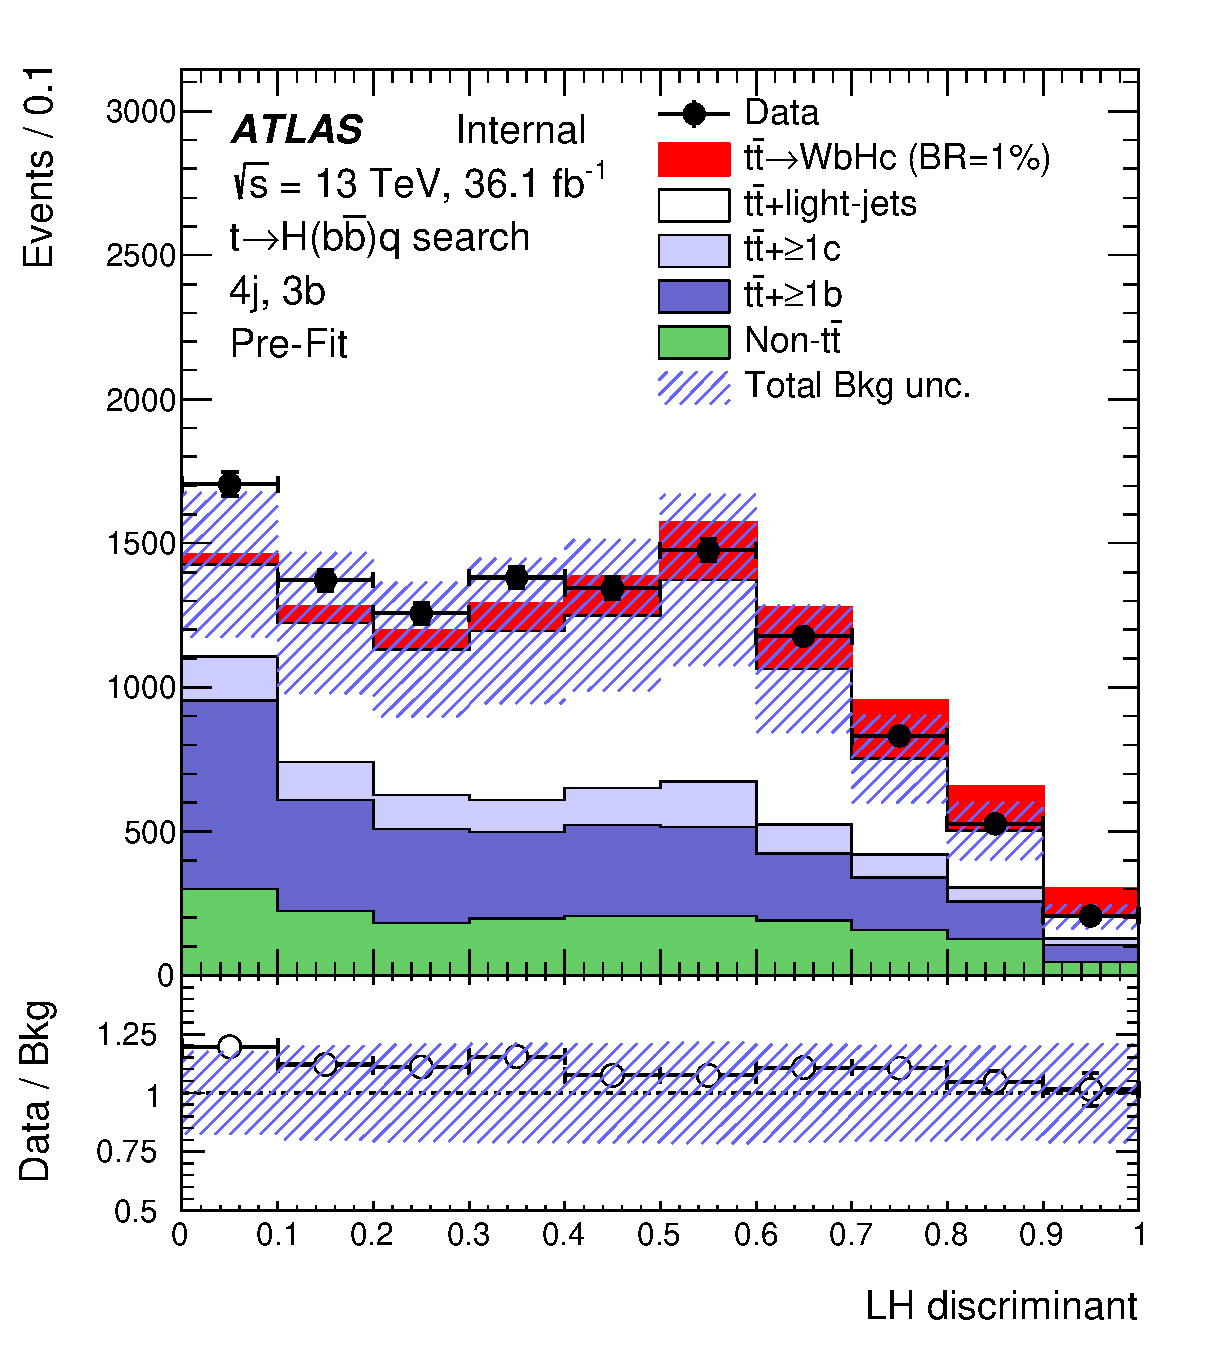
\includegraphics[width=0.33\textwidth]{figures/Hbb/fit/cH_plots//c1lep4jex3bex.eps}}
\subfloat[]{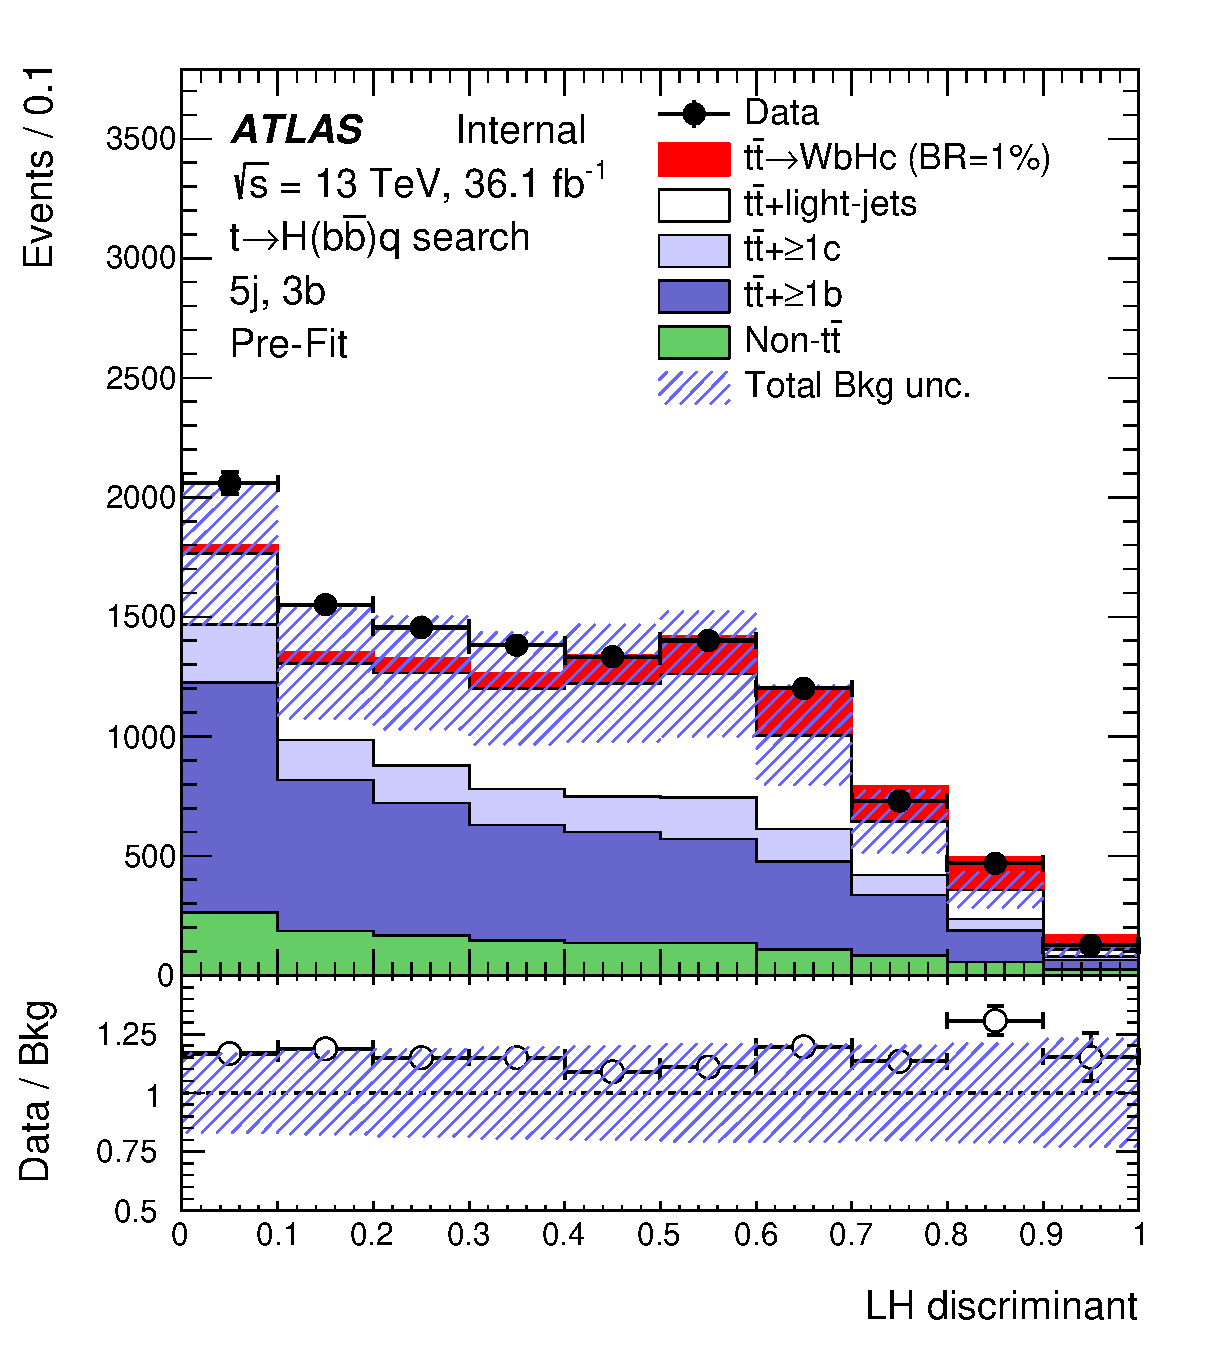
\includegraphics[width=0.33\textwidth]{figures/Hbb/fit/cH_plots//c1lep5jex3bex.eps}}
\subfloat[]{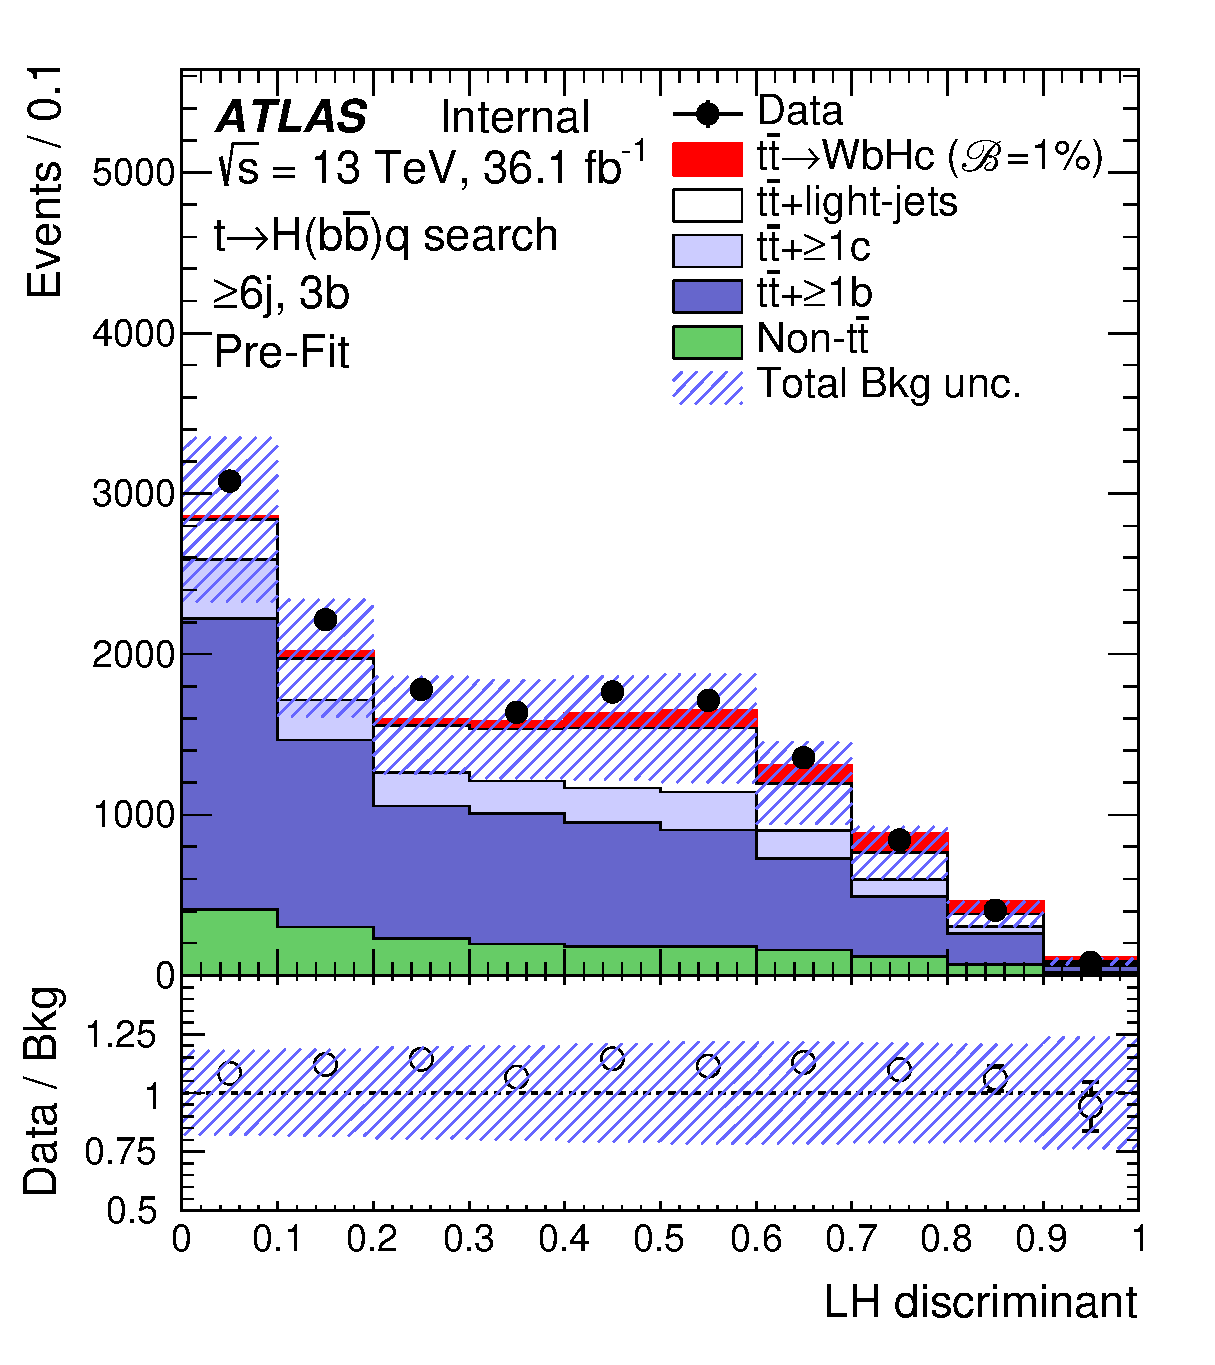
\includegraphics[width=0.33\textwidth]{figures/Hbb/fit/cH_plots//c1lep6jin3bex.eps}} \\
\subfloat[]{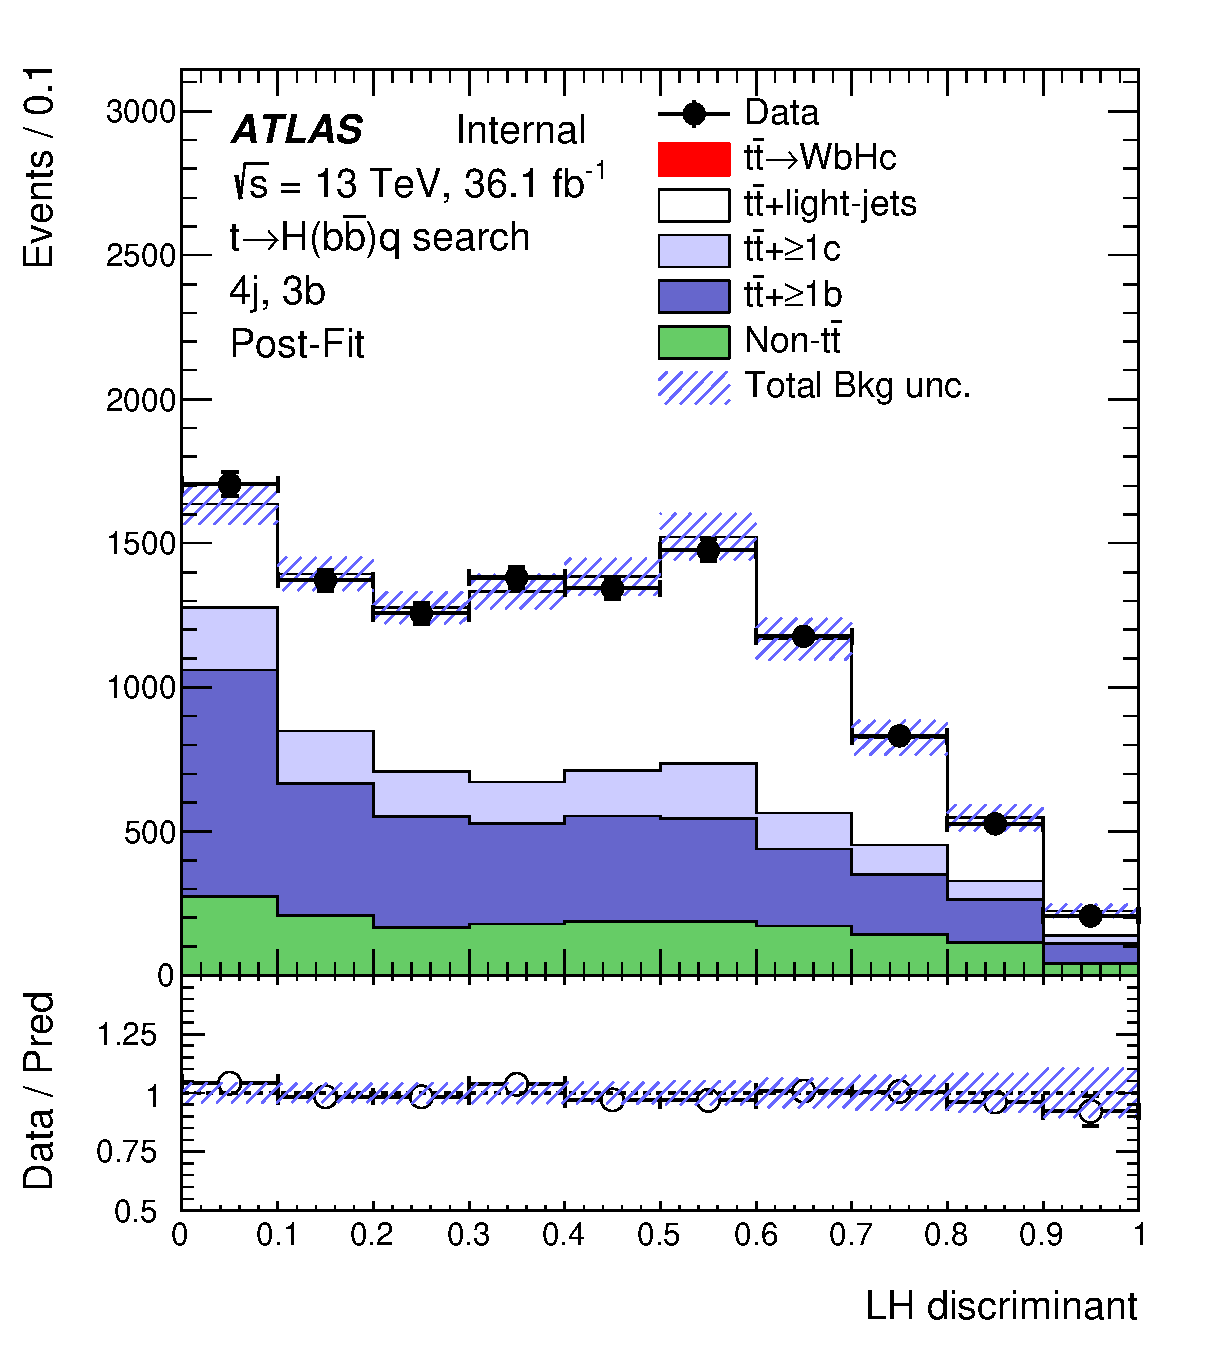
\includegraphics[width=0.33\textwidth]{figures/Hbb/fit/cH_plots//c1lep4jex3bex_postFit.eps}} 
\subfloat[]{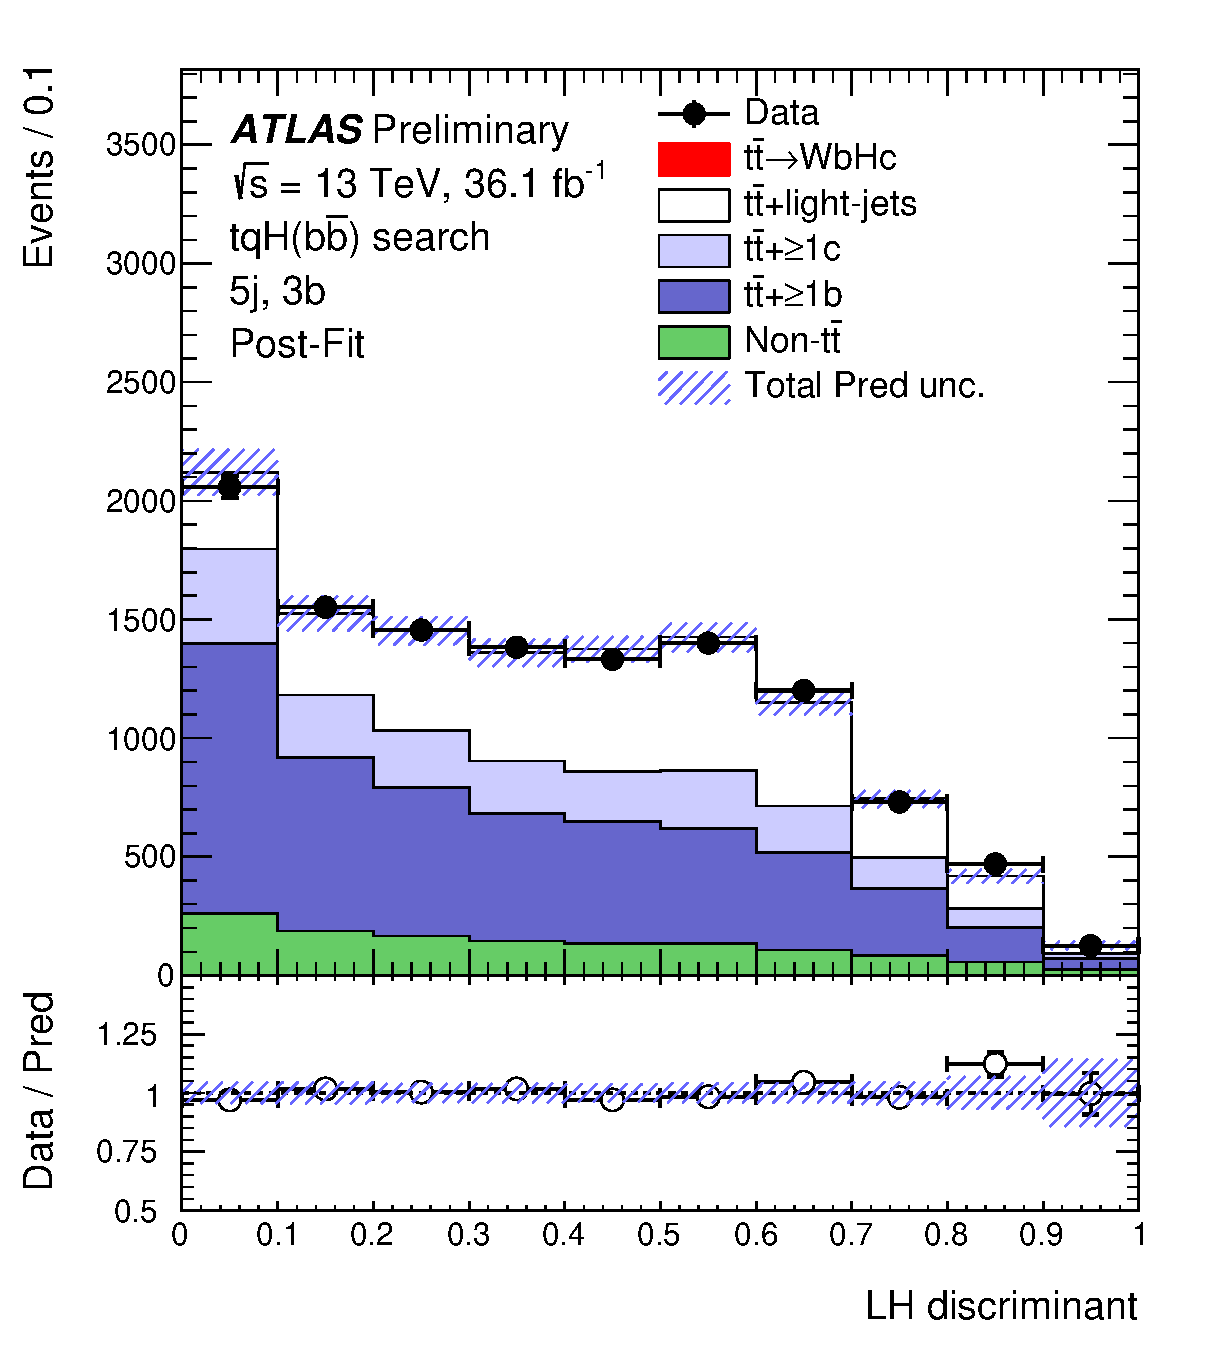
\includegraphics[width=0.33\textwidth]{figures/Hbb/fit/cH_plots//c1lep5jex3bex_postFit.eps}} 
\subfloat[]{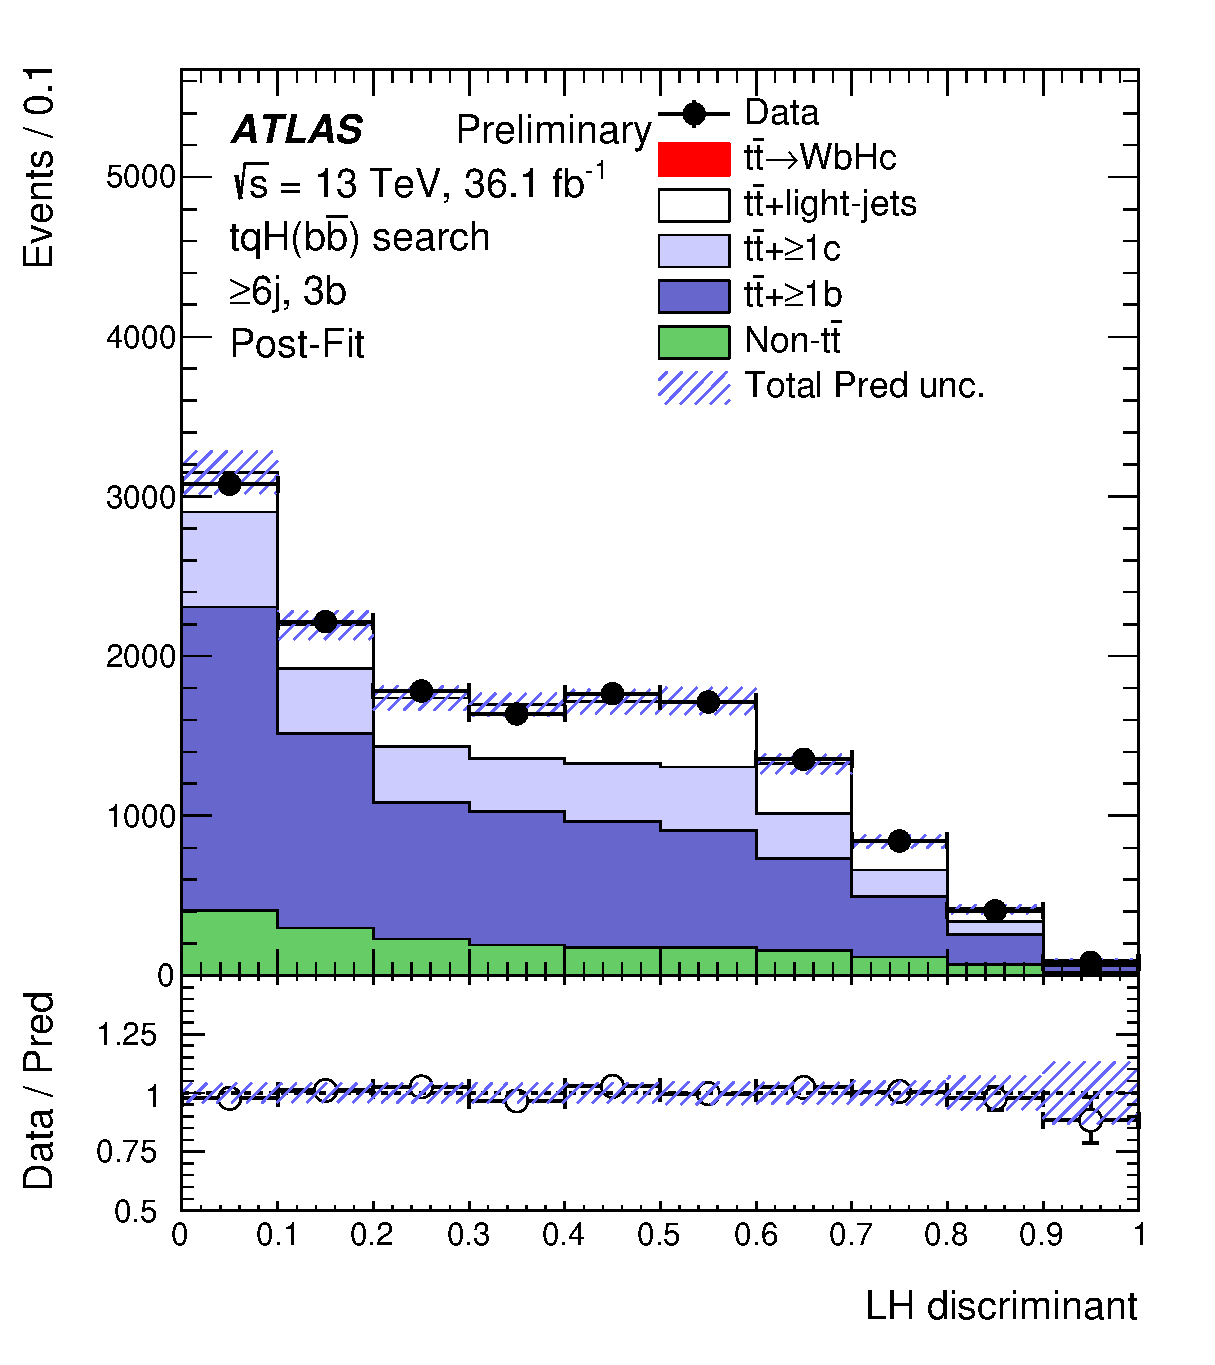
\includegraphics[width=0.33\textwidth]{figures/Hbb/fit/cH_plots//c1lep6jin3bex_postFit.eps}} \\
\caption{\small{$\Hbb$ search: Comparison between the data and prediction for the LH discriminant distribution in the 3b regions,
before and after performing the fit to data  (``Pre-Fit'' and ``Post-Fit'', respectively) under the signal-plus-background hypothesis.
Shown are the (4j, 3b) region (a) pre-fit and (d) post-fit,  the (5j, 3b) region (b) pre-fit and (e) post-fit, and
the ($\geq$6j, 3b) region (c) pre-fit and (f) post-fit.
The small contributions from $\ttbar V$, $\ttbar H$, single top, $W/Z$+jets, diboson, and multijet backgrounds are combined into a single background source 
referred to as ``Non-$\ttbar$''. 
In the pre-fit figures the expected $\Hc$ signal (solid red) corresponding to $\BR(t\to Hc)=1\%$ is also shown,
added on top of the background prediction. In the post-fit figures, the $\Hc$ signal has been scaled by its fitted signal strength.
%The bottom panel displays the ratio of data to the total prediction (``Pred''), which for the pre-fit figures includes only the total SM background,
%whereas for the post-fit figures includes the sum of the fitted signal and SM background.
The bottom panels display the ratios of data to either the SM background prediction before the fit (``Bkg'')  or the total signal-plus-background
prediction after the fit (``Pred''). 
%The blue triangles indicate points that are outside the vertical range of the figure. 
The hashed area represents the total uncertainty on the background.
In the case of the pre-fit background uncertainty, the normalisation uncertainty on the $\ttbin$ background is not included. }}
\label{fig:prepostfit_unblinded_WbHc_3btagex}
\end{center}
\end{figure*}
%%%%%%%%%%%%%%%%%%%%%%%%%%%%%%%%%%%%%%%

%%%%%%%%%%%%%%%%%%%%%%%%%%%%%%%%%%%%%%%
\begin{figure*}[htbp]
\begin{center}
\subfloat[]{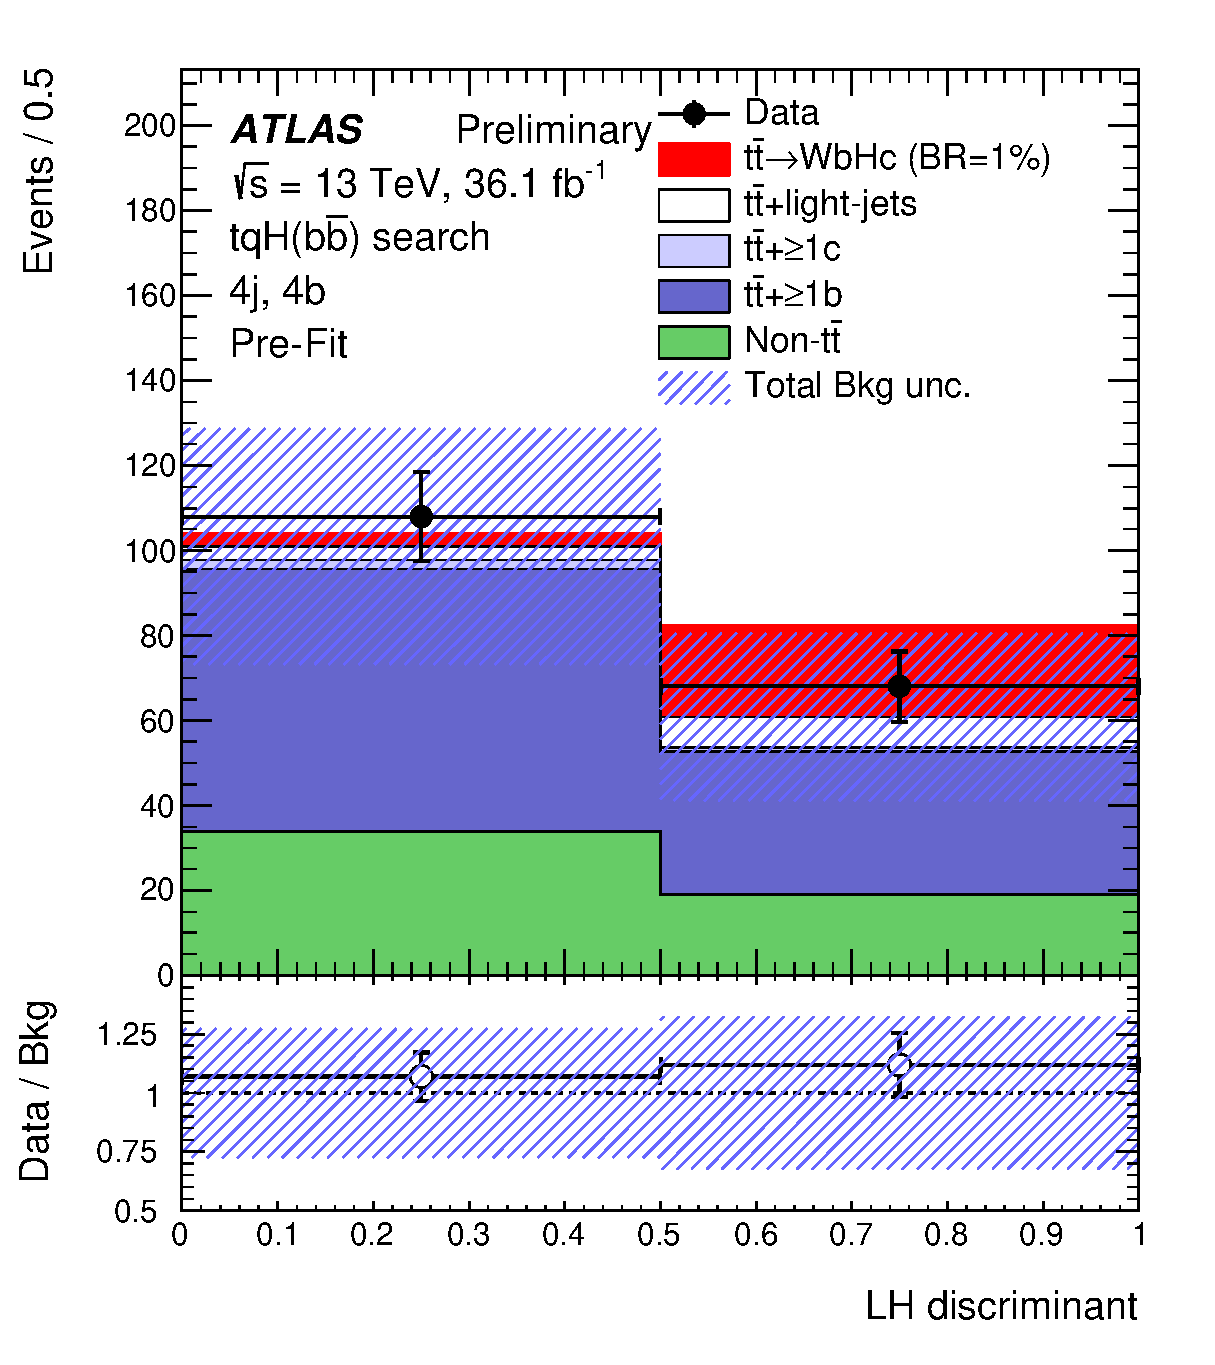
\includegraphics[width=0.33\textwidth]{figures/Hbb/fit/cH_plots//c1lep4jex4bin.eps}}
\subfloat[]{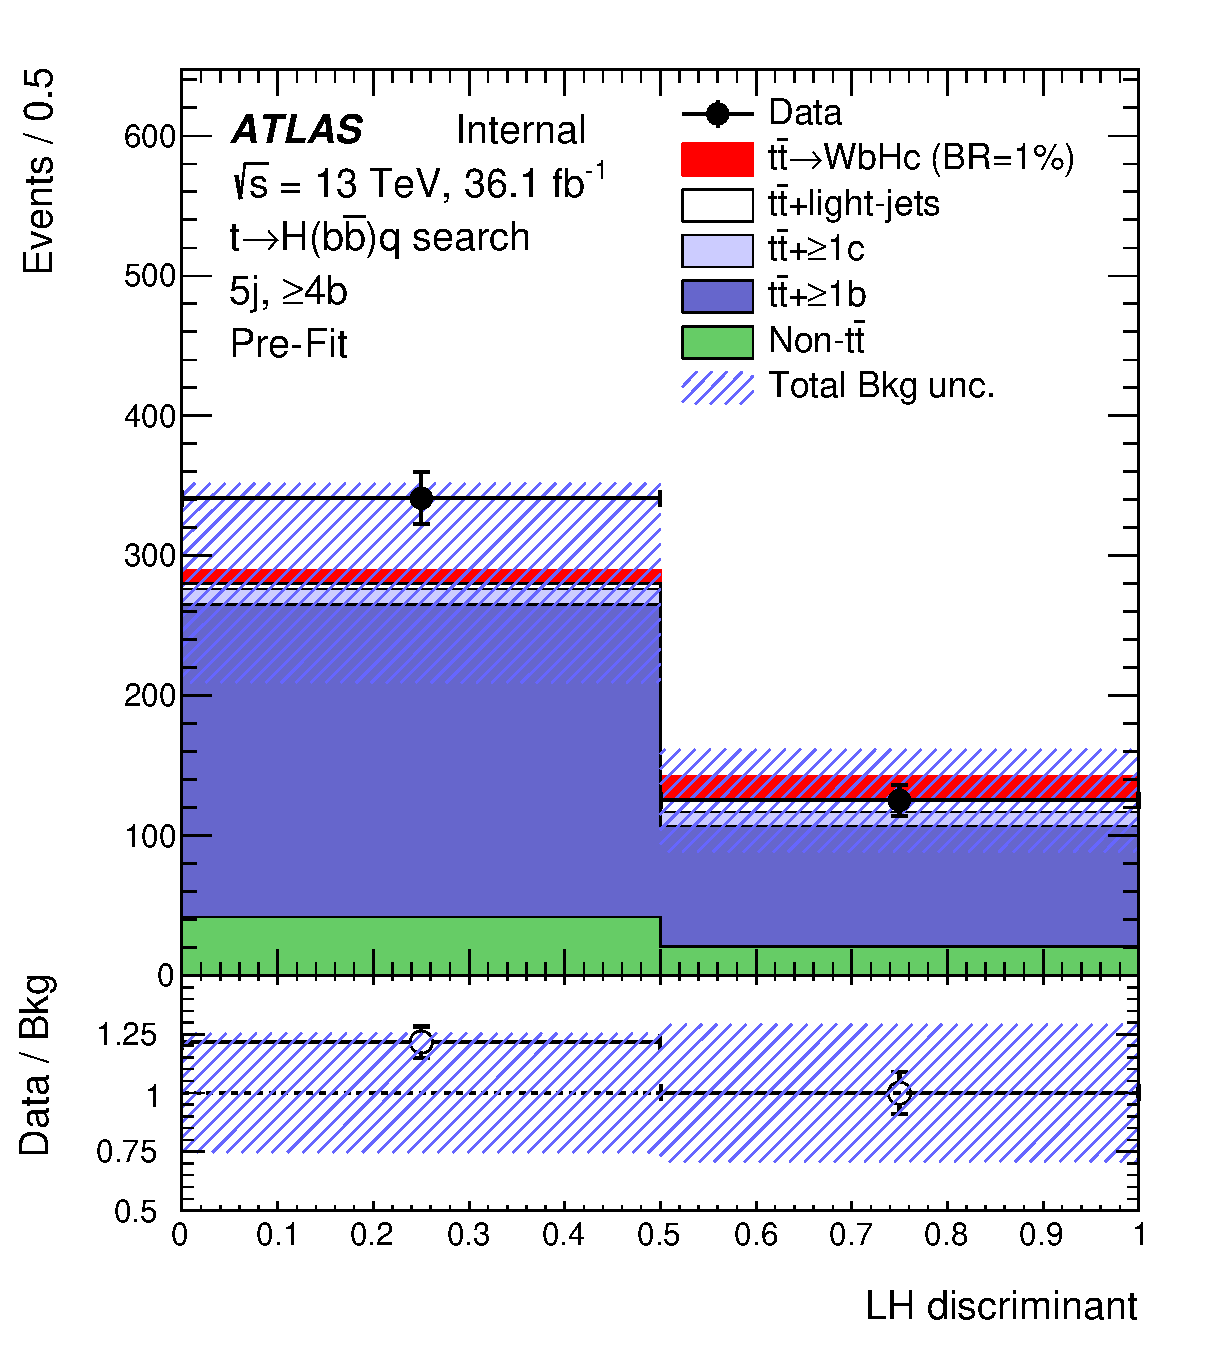
\includegraphics[width=0.33\textwidth]{figures/Hbb/fit/cH_plots//c1lep5jex4bin.eps}}
\subfloat[]{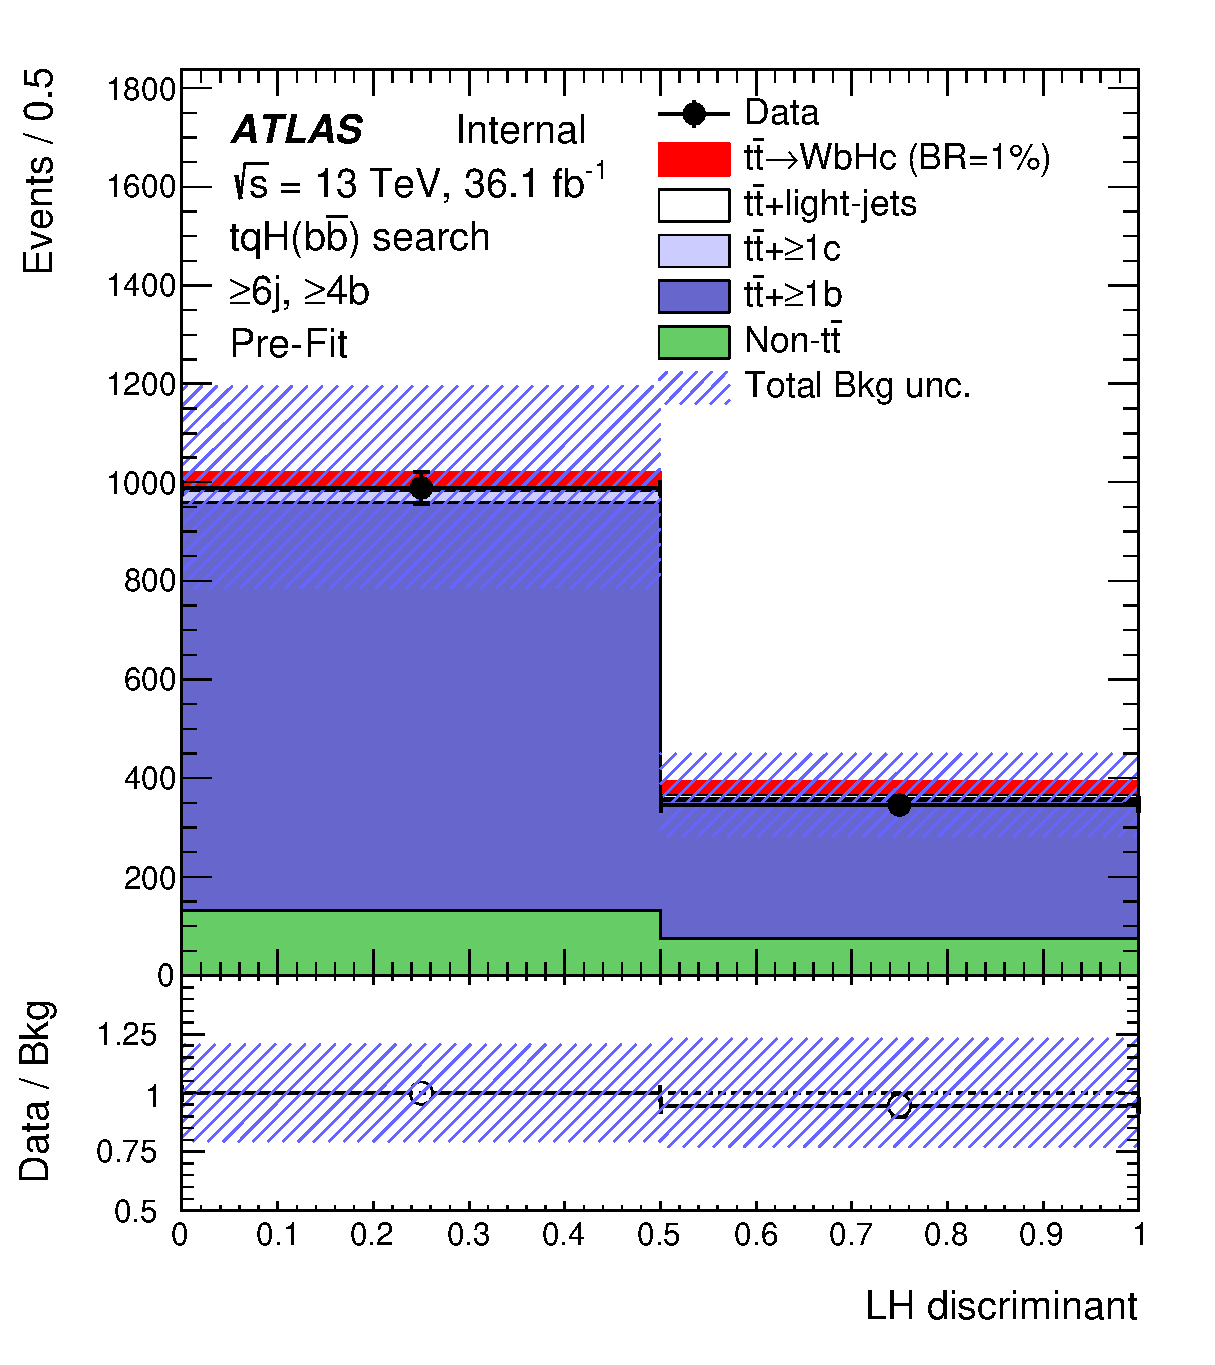
\includegraphics[width=0.33\textwidth]{figures/Hbb/fit/cH_plots//c1lep6jin4bin.eps}} \\
\subfloat[]{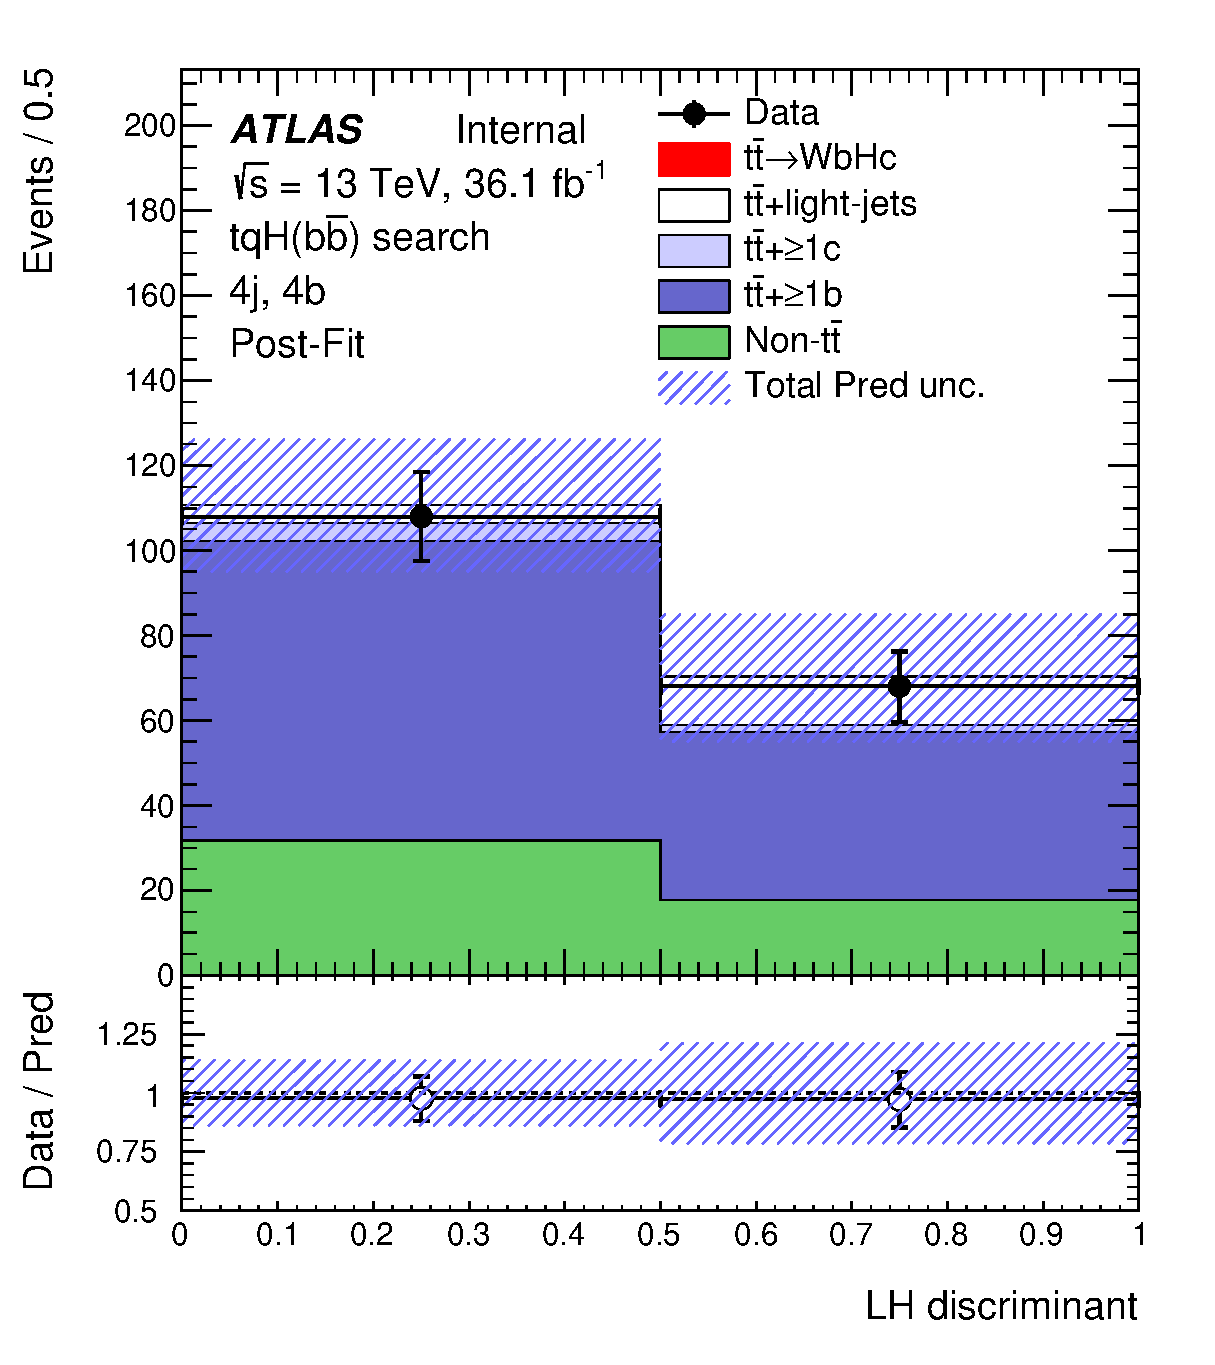
\includegraphics[width=0.33\textwidth]{figures/Hbb/fit/cH_plots//c1lep4jex4bin_postFit.eps}} 
\subfloat[]{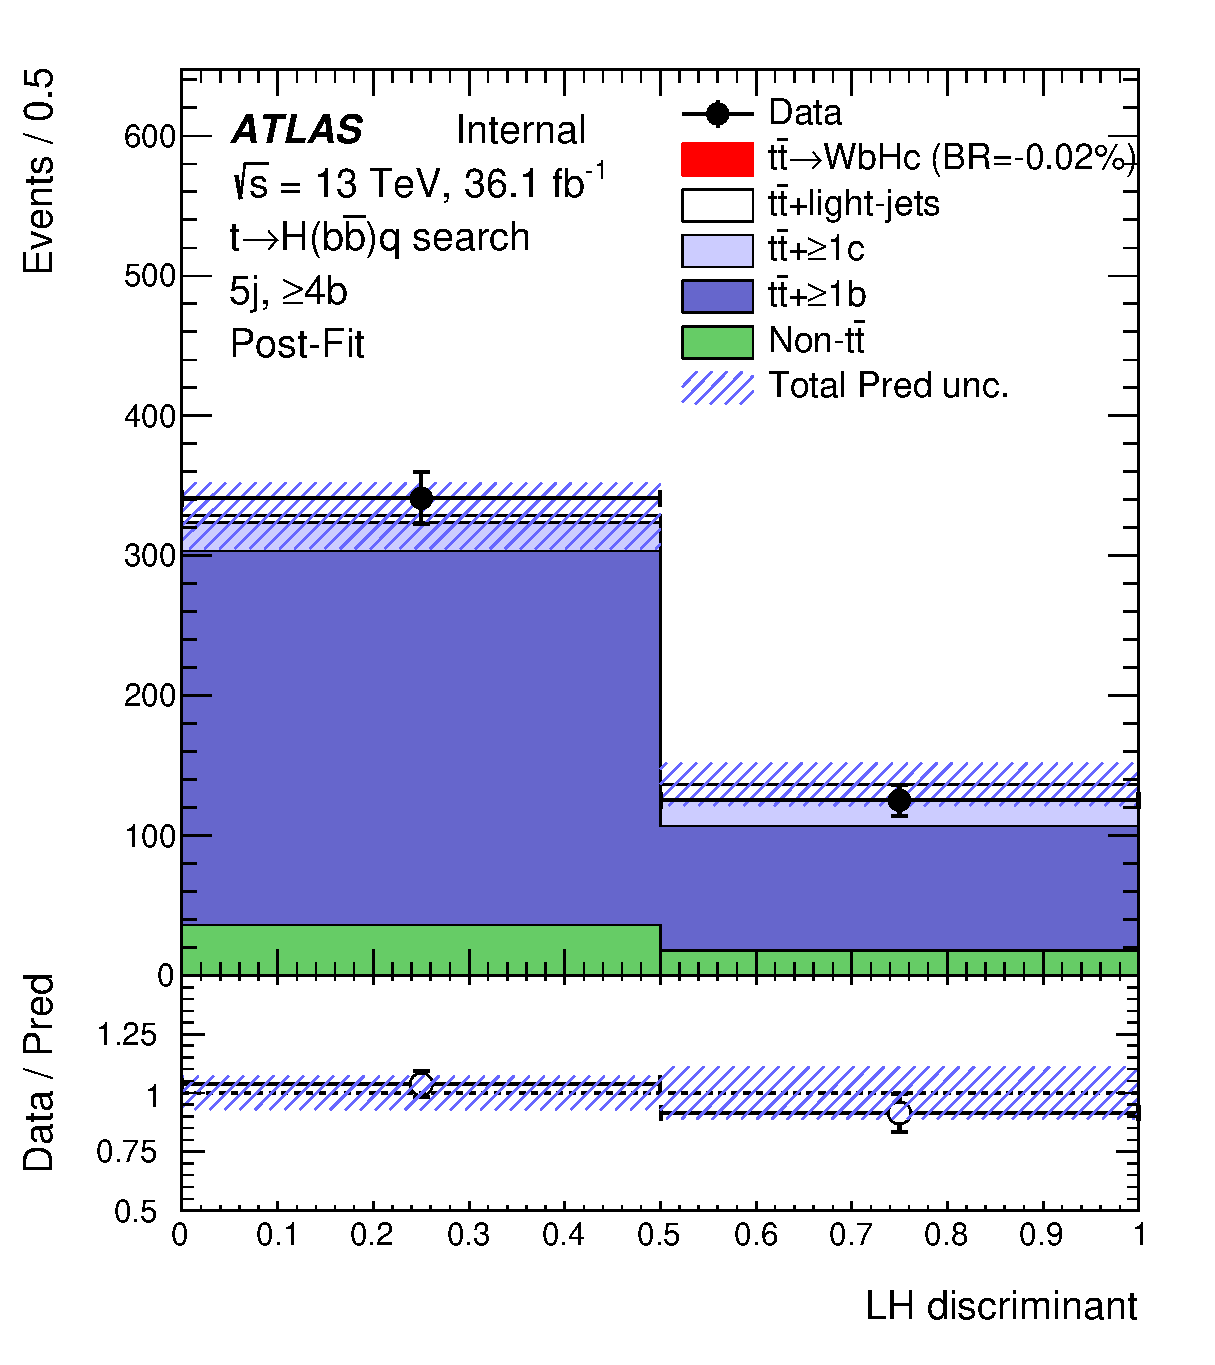
\includegraphics[width=0.33\textwidth]{figures/Hbb/fit/cH_plots//c1lep5jex4bin_postFit.eps}} 
\subfloat[]{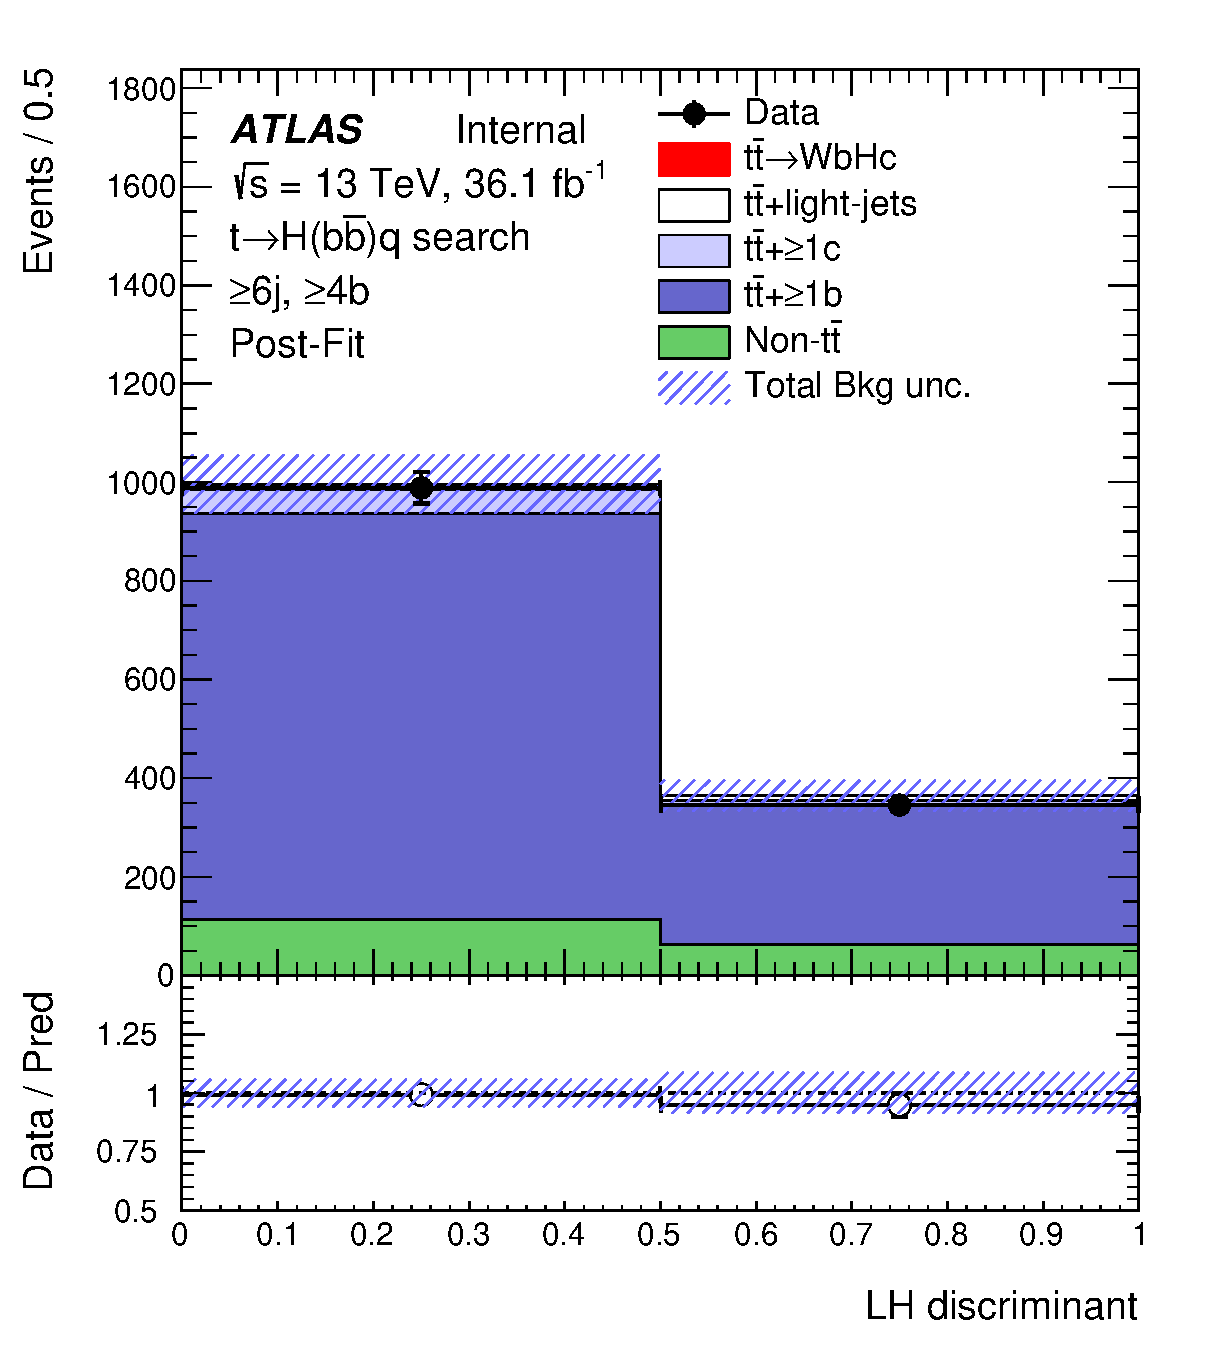
\includegraphics[width=0.33\textwidth]{figures/Hbb/fit/cH_plots//c1lep6jin4bin_postFit.eps}} \\
\caption{\small{$\Hbb$ search: Comparison between the data and prediction for the LH discriminant distribution in the $\geq$4b regions,
before and after performing the fit to data  (``Pre-Fit'' and ``Post-Fit'', respectively) under the signal-plus-background hypothesis.
Shown are the (4j, 4b) region (a) pre-fit and (d) post-fit,  the (5j, $\geq$4b) region (b) pre-fit and (e) post-fit, and
the ($\geq$6j, $\geq$4b) region (c) pre-fit and (f) post-fit.
The small contributions from $\ttbar V$, $\ttbar H$, single top, $W/Z$+jets, diboson, and multijet backgrounds are combined into a single background source 
referred to as ``Non-$\ttbar$''. 
In the pre-fit figures the expected $\Hc$ signal (solid red) corresponding to $\BR(t\to Hc)=1\%$ is also shown,
added on top of the background prediction. In the post-fit figures, the $\Hc$ signal has been scaled by its fitted signal strength.
%The bottom panel displays the ratio of data to the total prediction (``Pred''), which for the pre-fit figures includes only the total SM background,
%whereas for the post-fit figures includes the sum of the fitted signal and SM background.
The bottom panels display the ratios of data to either the SM background prediction before the fit (``Bkg'')  or the total signal-plus-background
prediction after the fit (``Pred''). 
%The blue triangles indicate points that are outside the vertical range of the figure. 
The hashed area represents the total uncertainty on the background.
In the case of the pre-fit background uncertainty, the normalisation uncertainty on the $\ttbin$ background is not included. }}
\label{fig:prepostfit_unblinded_WbHc_4btagin}
\end{center}
\end{figure*}
%%%%%%%%%%%%%%%%%%%%%%%%%%%%%%%%%%%%%%%

%
%%%%%%%%%%%%%%%%%%%%%%%%%%%%%%%%%%%%%%%%
%\begin{figure*}[htbp!]
%\begin{center}
%\includegraphics[width=0.60\textwidth]{figures/fig07.pdf}
%\caption{\small {$\Hcbb$ search: the fitted values of the nuisance parameters for the most important sources
%of systematic uncertainty and their impact on the measured signal strength. 
%The points, which are drawn conforming to the scale of the bottom axis, show the deviation of each of the 
%fitted nuisance parameters, $\hat\mathrm{{\theta}}$, from $\rm{\theta_{0}}$, which is the nominal value of that nuisance 
%parameter, in units of the pre-fit standard deviation $\Delta\theta$.
%The error bars show the post-fit uncertainties, 
%$\sigma_{\theta}$, which are close to 1 if the data do not provide any further constraint on that uncertainty.
%Conversely, a value of $\sigma_{\theta}$ much smaller than 1 indicates a significant reduction with respect to 
%the original uncertainty. The nuisance parameters are sorted according to their post-fit effect on 
%$\mu$ (hashed blue area), conforming to the scale of the top axis, with those with the largest impact at the top. }}
%\label{fig:ranking_bb_Hc}
%\end{center}
%\end{figure*}
%%%%%%%%%%%%%%%%%%%%%%%%%%%%%%%%%%%%%%%%

\subsection{$\Htautau$ search}
\label{sec:results_Htautau}

A binned likelihood fit under the signal-plus-background hypothesis is performed to the BDT discriminant distributions in the four 
analysis regions considered (see Section~\ref{sec:strategy_Htautau}). The unconstrained parameters of the fit are the signal 
strength, as well as four independent parameters associated with the normalisation of the fake $\tauhad$ background in each of the analysis regions. 
Figure~\ref{fig:prepostfit_unblinded_WbHc_lh} shows a comparison of the data and prediction for the BDT discriminant distribution in
the ($\lephad$, 3j) and ($\lephad$, $\geq$4j) regions, both pre- and post-fit to data, in the case of the $\Hc$ search.  
A similar comparison for the ($\hadhad$, 3j) and ($\hadhad$, $\geq$4j) regions can be found in Figure~\ref{fig:prepostfit_unblinded_WbHc_hh}.
The post-fit yields can be found in Appendix~\ref{sec:prepostfit_yields_Htautau_appendix}.
The best-fit branching ratio obtained is $\BR(t\to Hc)=[-4.4^{+9.9}_{-8.5}\,(\mathrm{stat+syst})] \times 10^{-4}$, assuming that $\BR(t\to Hu)=0$. 
A similar fit is performed for the $\Hu$ search, yielding $\BR(t\to Hu)=[-5.3^{+9.1}_{-7.8}\,(\mathrm{stat+syst})] \times 10^{-4}$,
assuming that $\BR(t\to Hc)=0$. In both cases, the uncertainty in the measured branching ratio is dominated by the statistical uncertainty.
The main contributions to the total systematic uncertainty arise from the fake $\tauhad$ background estimation and the uncertainty associated
with the different response of the detector the quark-initiated and gluon-initiated jets.
No significant excess in data above the background expectation is found, 
and observed (expected) 95\% CL limits are set on $\BR(t\to Hc)$ and $\BR(t\to Hu)$:
$\BR(t\to Hc)<1.9 \times 10^{-3}\,(2.1 \times 10^{-3})$ and $\BR(t\to Hu)<1.7 \times 10^{-3}\,(2.0 \times 10^{-3})$.

%%%%%%%%%%%%%%%%%%%%%%%%%%%%%%%%%%%%%%%
\begin{figure*}[htbp]
\begin{center}
\subfloat[]{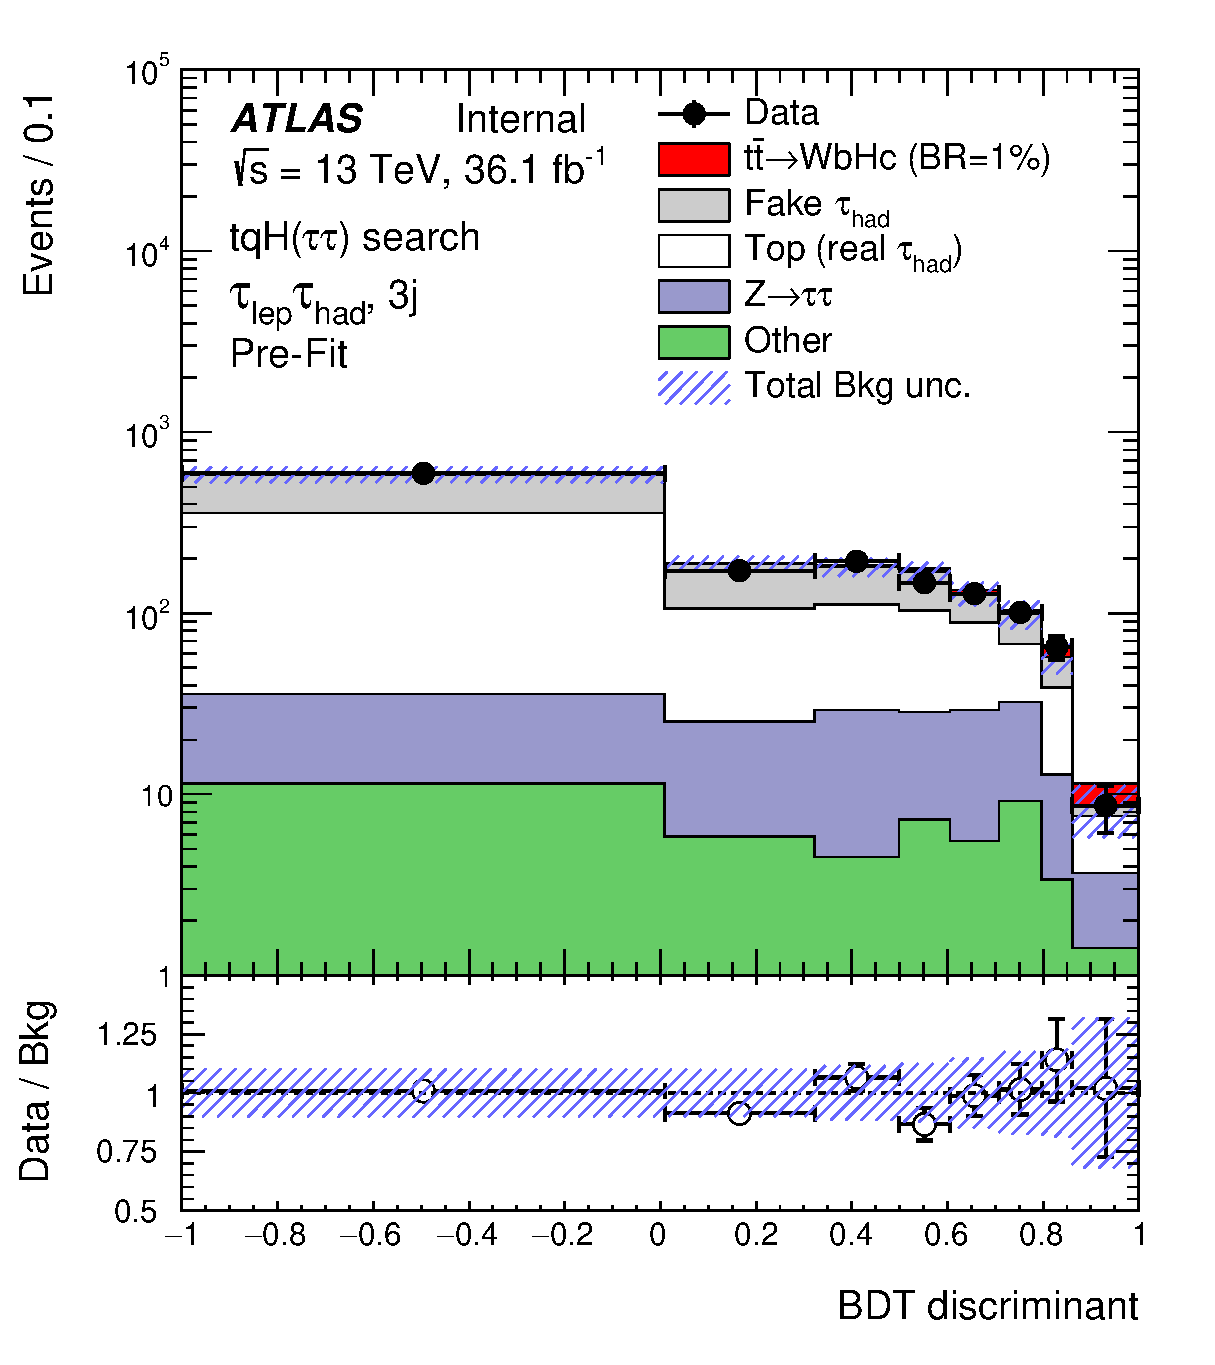
\includegraphics[width=0.40\textwidth]{figures/Htautau/fit/lephad_3j_FR.eps}}
\subfloat[]{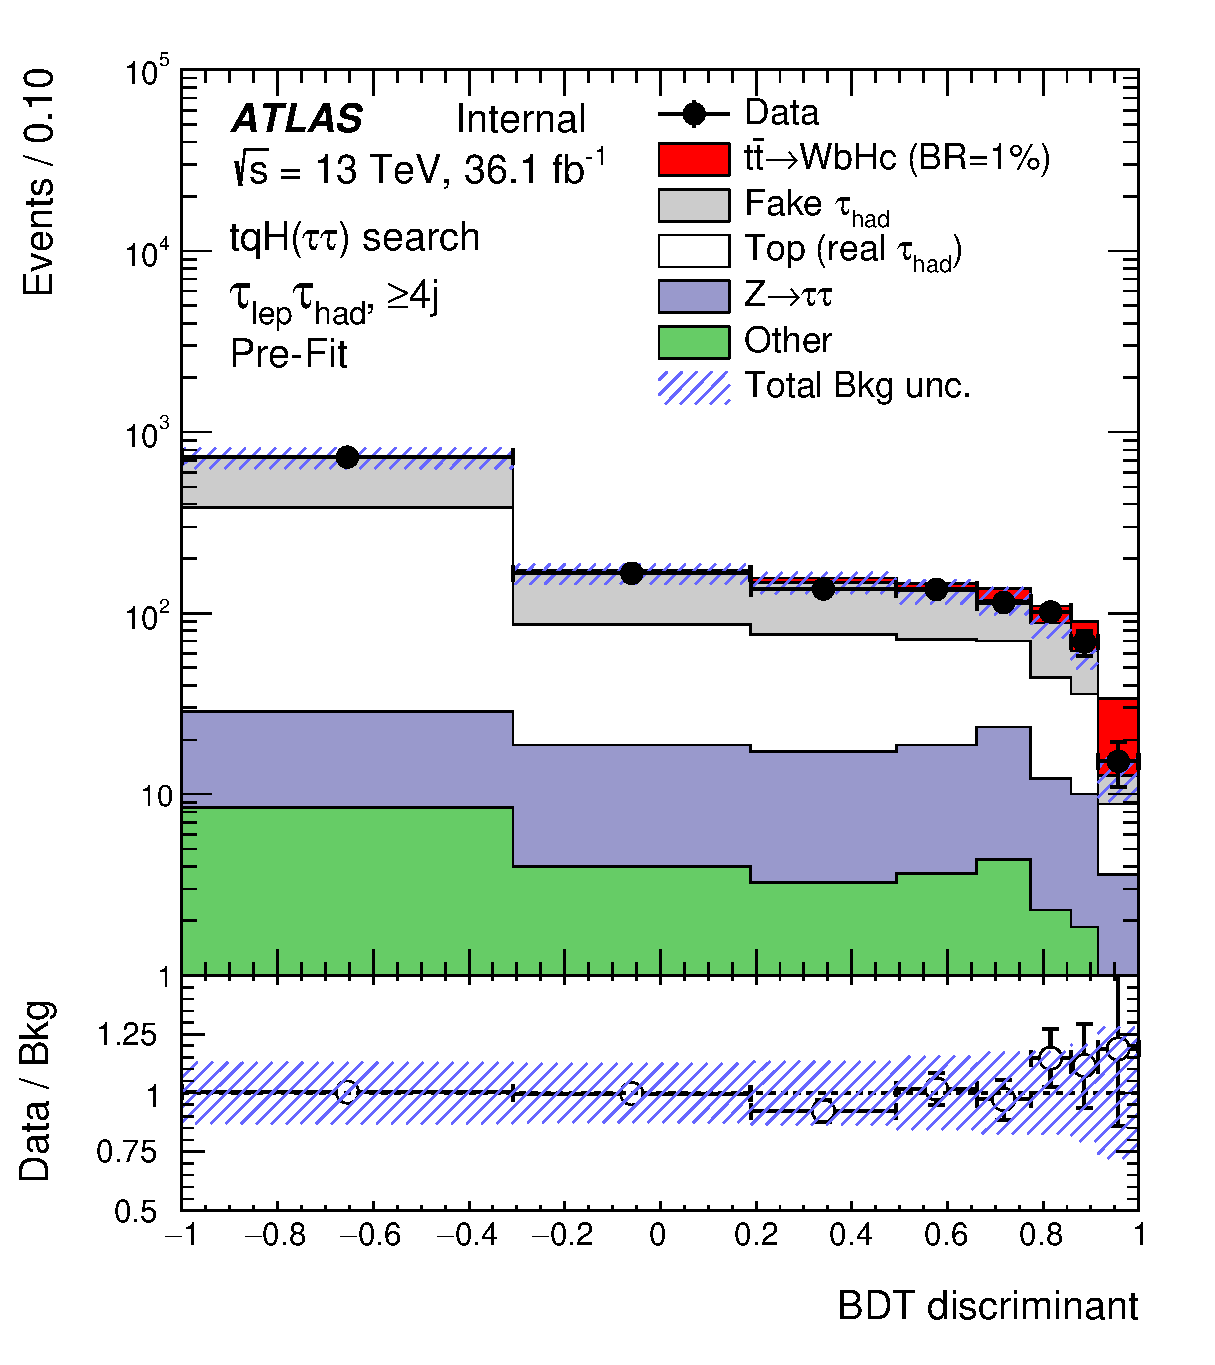
\includegraphics[width=0.40\textwidth]{figures/Htautau/fit/lephad_4j_FR.eps}} \\
\subfloat[]{\includegraphics[width=0.40\textwidth]{figures/Htautau/fit/lephad_3j_FR_postfit.eps}}
\subfloat[]{\includegraphics[width=0.40\textwidth]{figures/Htautau/fit/lephad_4j_FR_postfit.eps}} \\
\caption{\small{$\Htautau$ search: Comparison between the data and prediction for the BDT discriminant distribution in the
$\lephad$ channel, before and after performing the fit to data  (``Pre-Fit'' and ``Post-Fit'', respectively) under the signal-plus-background hypothesis.
Shown are the ($\lephad$, 3j) region (a) pre-fit and (c) post-fit, and the ($\lephad$, $\geq$4j) region (b) pre-fit and (d) post-fit.
The small contributions from $\ttbar V$, $\ttbar H$, single top, $Z\to \ell^+\ell^-$ ($\ell = e, \mu$), and diboson backgrounds are combined 
into a single background source referred to as ``Other''. 
In the pre-fit figures the expected $\Hc$ signal (solid red) corresponding to $\BR(t\to Hc)=1\%$ is also shown,
added on top of the background prediction. In the post-fit figures, the $\Hc$ signal has been scaled by its fitted signal strength.
%The bottom panel displays the ratio of data to the total prediction (``Pred''), which for the pre-fit figures includes only the total SM background,
%whereas for the post-fit figures includes the sum of the fitted signal and SM background.
The bottom panels display the ratios of data to either the SM background prediction before the fit (``Bkg'')  or the total signal-plus-background
prediction after the fit (``Pred''). 
%The blue triangles indicate points that are outside the vertical range of the figure. 
The hashed area represents the total uncertainty on the background. }}
\label{fig:prepostfit_unblinded_WbHc_lh}
\end{center}
\end{figure*}
%%%%%%%%%%%%%%%%%%%%%%%%%%%%%%%%%%%%%%%

%%%%%%%%%%%%%%%%%%%%%%%%%%%%%%%%%%%%%%%
\begin{figure*}[htbp]
\begin{center}
\subfloat[]{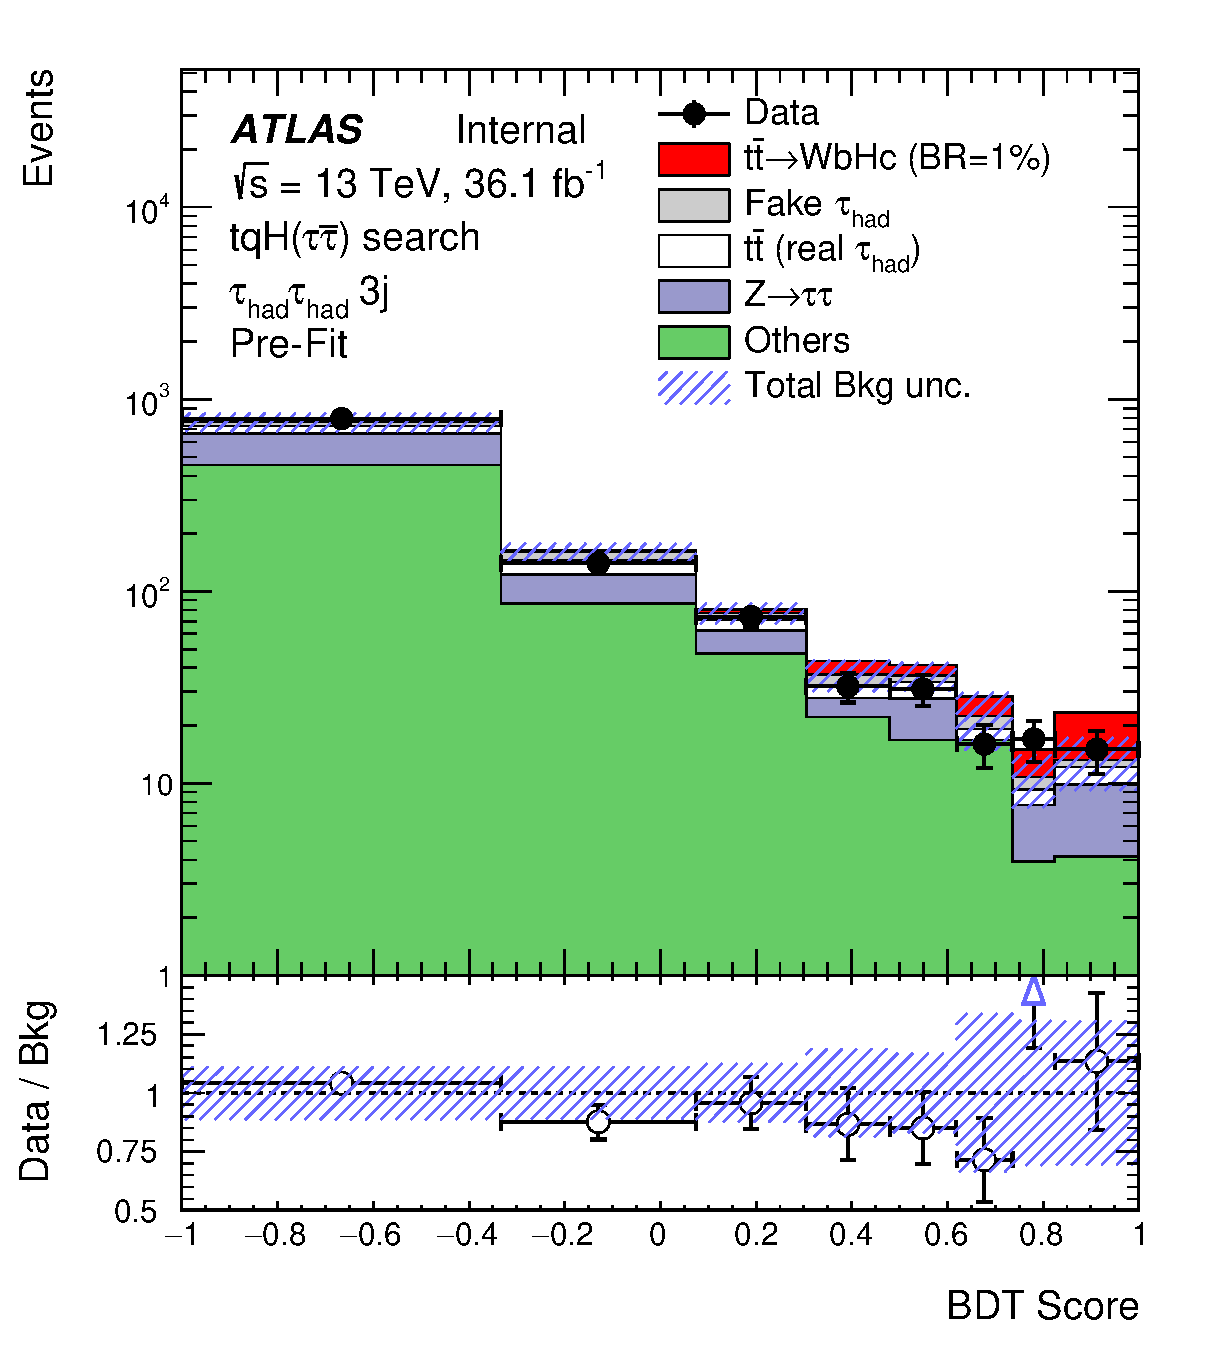
\includegraphics[width=0.40\textwidth]{figures/Htautau/fit/hadhad_3j_FR.eps}}
\subfloat[]{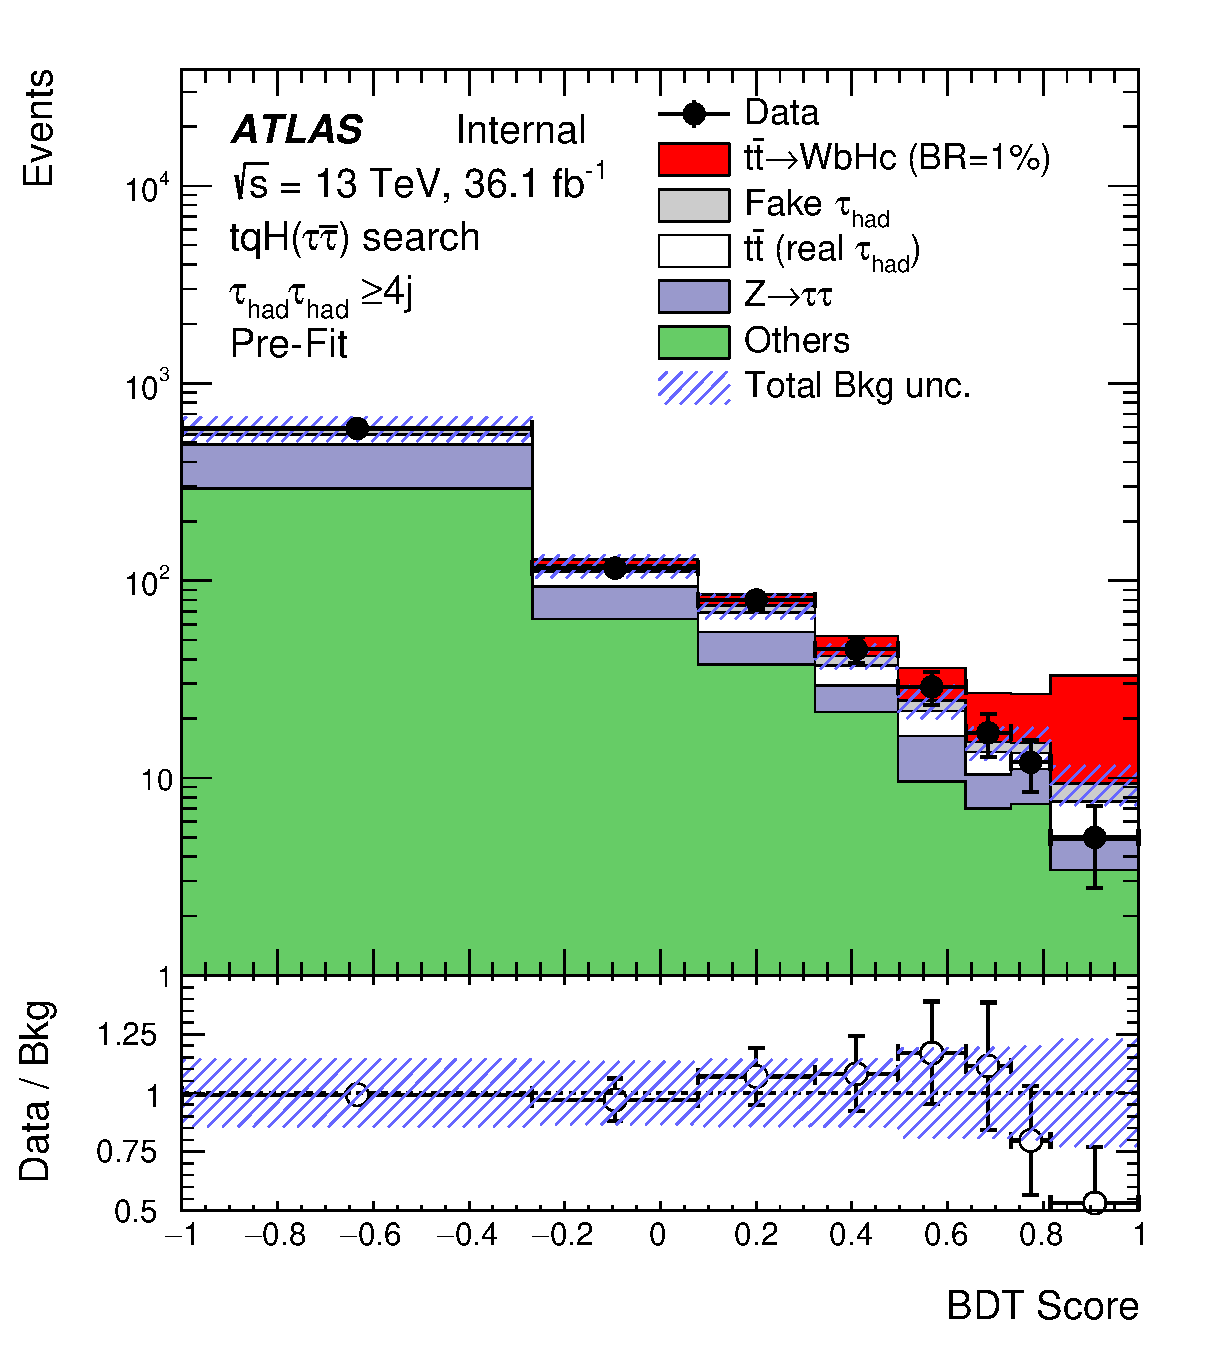
\includegraphics[width=0.40\textwidth]{figures/Htautau/fit/hadhad_4j_FR.eps}} \\
\subfloat[]{\includegraphics[width=0.40\textwidth]{figures/Htautau/fit/hadhad_3j_FR_postfit.eps}}
\subfloat[]{\includegraphics[width=0.40\textwidth]{figures/Htautau/fit/hadhad_4j_FR_postfit.eps}} \\
\caption{\small{$\Htautau$ search: Comparison between the data and prediction for the BDT discriminant distribution in the 
$\hadhad$ channel, before and after performing the fit to data  (``Pre-Fit'' and ``Post-Fit'', respectively) under the signal-plus-background hypothesis.
Shown are the ($\hadhad$, 3j) region (a) pre-fit and (c) post-fit, and the ($\hadhad$, $\geq$4j) region (b) pre-fit and (d) post-fit.
The small contributions from $\ttbar V$, $\ttbar H$, single top, $Z\to \ell^+\ell^-$ ($\ell = e, \mu$), and diboson backgrounds are combined 
into a single background source referred to as ``Other''. 
In the pre-fit figures the expected $\Hc$ signal (solid red) corresponding to $\BR(t\to Hc)=1\%$ is also shown,
added on top of the background prediction. In the post-fit figures, the $\Hc$ signal has been scaled by its fitted signal strength.
%The bottom panel displays the ratio of data to the total prediction (``Pred''), which for the pre-fit figures includes only the total SM background,
%whereas for the post-fit figures includes the sum of the fitted signal and SM background.
The bottom panels display the ratios of data to either the SM background prediction before the fit (``Bkg'')  or the total signal-plus-background
prediction after the fit (``Pred''). 
The blue triangles indicate points that are outside the vertical range of the figure. 
The hashed area represents the total uncertainty on the background. }}
\label{fig:prepostfit_unblinded_WbHc_hh}
\end{center}
\end{figure*}
%%%%%%%%%%%%%%%%%%%%%%%%%%%%%%%%%%%%%%%

\subsection{Combination of ATLAS searches}
\label{sec:results_combo}

The $\Hbb$ and $\Htautau$ searches discussed previously are combined with ATLAS searches in 
diphoton~\cite{Aaboud:2017mfd} and multilepton~\cite{Aaboud:2018pob} final states using the same data set, 
denoted as ``$\Hgg$ search" and ``$\HML$ search", respectively.
In this combination, the only systematic uncertainties taken to be fully correlated among the four searches are 
those affecting the integrated luminosity, the $\ttbar$ cross section, signal modelling, a subset of the uncertainties
on the Higgs boson branching ratios (those associated with uncertainties on $\alpha_\mathrm{S}$ and $m_b$), 
and a subset of jet-related uncertainties (jet energy resolution and JVT requirement). 
The rest of jet-related uncertainties (jet energy scale and $b$-tagging) are taken as fully correlated among 
the $\Hbb$, $\Htautau$, and $\HML$ searches, but uncorrelated with the $\Hgg$ search, due to the different
uncertainty breakdown used. The rest of uncertainties, e.g. those related to leptons and to background modelling, are taken
as uncorrelated among the four searches. These assumptions are justified by the different lepton selection and $\pt$ cuts, 
as well as the different background composition and background estimation techniques, used by the searches.
Since all searches,  with the exception of the $\Hbb$ search, are dominated 
by the data statistics, the effect of these assumptions in the final result is found to be negligible.

%%The uncertainties on the Higgs boson branching ratios primarily affect the $\Hgg$ and $\Hbb$ searches.  
%Other uncertainties such as those associated with leptons,
%jet energy scale and $b$-tagging should be partially correlated among the searches, but the differences in treatment 
%between analyses (different lepton selection and $\pt$ cuts, different uncertainty breakdown for jet energy scale and 
%different $b$-tagging efficiency working points are used) make it difficult to account for correlations. 
%However, since all searches, 
%with the exception of the $\Hbb$ search, are dominated by the data statistics, the effect of this simplification is negligible.

The first set of combined results is obtained for each branching ratio separately, setting the other branching ratio to zero.
The best-fit combined branching ratios are $\BR(t\to Hc)=[3.0^{+4.0}_{-3.4}\,(\mathrm{stat+syst})] \times 10^{-4}$ and 
$\BR(t\to Hu)=[4.2^{+4.2}_{-3.6}\,(\mathrm{stat+syst})] \times 10^{-4}$.  
%The difference between the central values of $\BR(t\to Hc)$ and $\BR(t\to Hu)$ originates from the ability of the $H \to b\bar{b}$ search to 
%probe both decay modes separately.
A comparison of the best-fit branching ratios for the individual searches and their combination can be found in Figure~\ref{fig:summary_printnum_hc} 
for $\BR(t\to Hc)$ and Figure~\ref{fig:summary_printnum_hu} for $\BR(t\to Hu)$.
The observed (expected) 95\% CL combined upper limits on the branching ratios are 
$\BR(t\to Hc)<1.1 \times 10^{-3}\,(8.3 \times 10^{-4})$ and $\BR(t\to Hu)<1.2 \times 10^{-3}\,(8.3 \times 10^{-4})$
A summary of the upper limits on the branching ratios obtained by the individual searches, as well as their combination, 
can be found in Table~\ref{tab:limits_summary}, as is displayed in Figure~\ref{fig:limits_combo_1D}. 

Upper limits on the branching ratios $\BR(t\to Hq)$ ($q=u,c$) can be translated to upper limits on the non-flavour-diagonal Yukawa couplings $\lamHq$ 
appearing in the following Lagrangian~\cite{Harnik:2012pb}:
\begin{equation}
{\cal L}_\mathrm{FCNC} = -\lambda_{t_L q_R} \bar{t}_L q_R H - \lambda_{q_L t_R} \bar{q}_L t_R H  + h.c.
\end{equation}
The branching ratio $\BR(t\to Hq)$ is estimated as the ratio of its partial width~\cite{Zhang:2013xya} to the SM $t \to Wb$ partial width~\cite{Denner:1990ns}, 
which is assumed to be dominant. Both predicted partial widths include next-to-leading-order (NLO) QCD corrections.
Using the expression derived in Ref.~\cite{Aad:2014dya}, the coupling $|\lamHq|$ can be extracted as $| \lamHq | = (1.92 \pm 0.02) \sqrt{\BR(t\to Hq)}$.
The $\lamHq$ coupling corresponds to the sum in quadrature of the couplings relative to the two possible chirality combinations of the quark fields, 
$\lamHq \equiv \sqrt{ |\lambda_{t_Lq_R}|^2 +   |\lambda_{q_L t_R}|^2 }$~\cite{Harnik:2012pb}.
The observed (expected) upper limits on the couplings from the combination of the searches are $|\lamHc|<0.064\,(0.055)$ and $|\lamHu|<0.066\,(0.055)$.

%Since each of the searches has slightly different sensitivity to the two branching ratios, a simultaneous fit is performed for the combination of all searches.
%The best-fit branching ratios obtained from the simultaneous fit are 
%$\BR(t\to Hc)=[0.XX \pm 0.XX\,(\mathrm{ stat.}) \pm 0.XX\,(\mathrm{ syst.})]\%$ and 
%$\BR(t\to Hu)=[0.XX \pm 0.XX\,(\mathrm{ stat.}) \pm 0.XX\,(\mathrm{ syst.})]\%$, with a correlation coefficient of $-0.XX$, 
%as shown in Figure~\ref{fig:nllscan_combo_2D}.
A similar set of results can be obtained by  simultaneously probing both branching ratios. 
Figure~\ref{fig:limits_combo_2D}(a) shows the 95\% CL upper limits on the branching ratios in the $\BR(t\to Hu)$ versus $\BR(t\to Hc)$ plane. 
%\textbf{Add comment of what discriminant is used in this case and the caveat regarding the corresponding 1D limit.}
The corresponding upper limits on the couplings in the $|\lamHu|$ versus $|\lamHc|$ plane can be found in Figure~\ref{fig:limits_combo_2D}(b).

%%%%%%%%%%%%%%
\begin{figure*}[t!]
\begin{center}
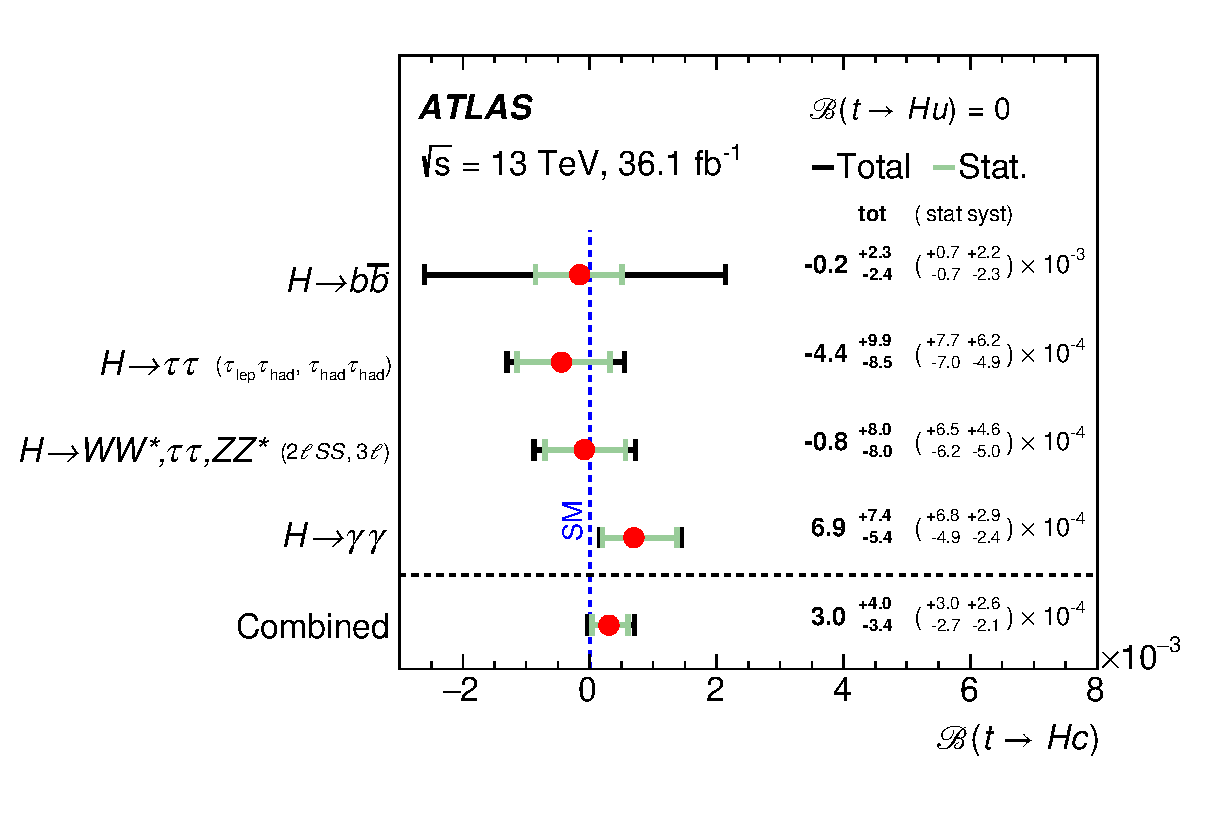
\includegraphics[width=0.6\textwidth]{figures/Combo/POI.eps}
\caption{\small {Summary of the best-fit $\BR(t\to Hc)$ for the individual searches as well as their combination,
assuming that $\BR(t\to Hu)=0$. }}
\label{fig:summary_printnum_hc} 
\end{center}
\end{figure*}
%%%%%%%%%%%%%%
%%%%%%%%%%%%%%
\begin{figure*}[h!]
\begin{center}
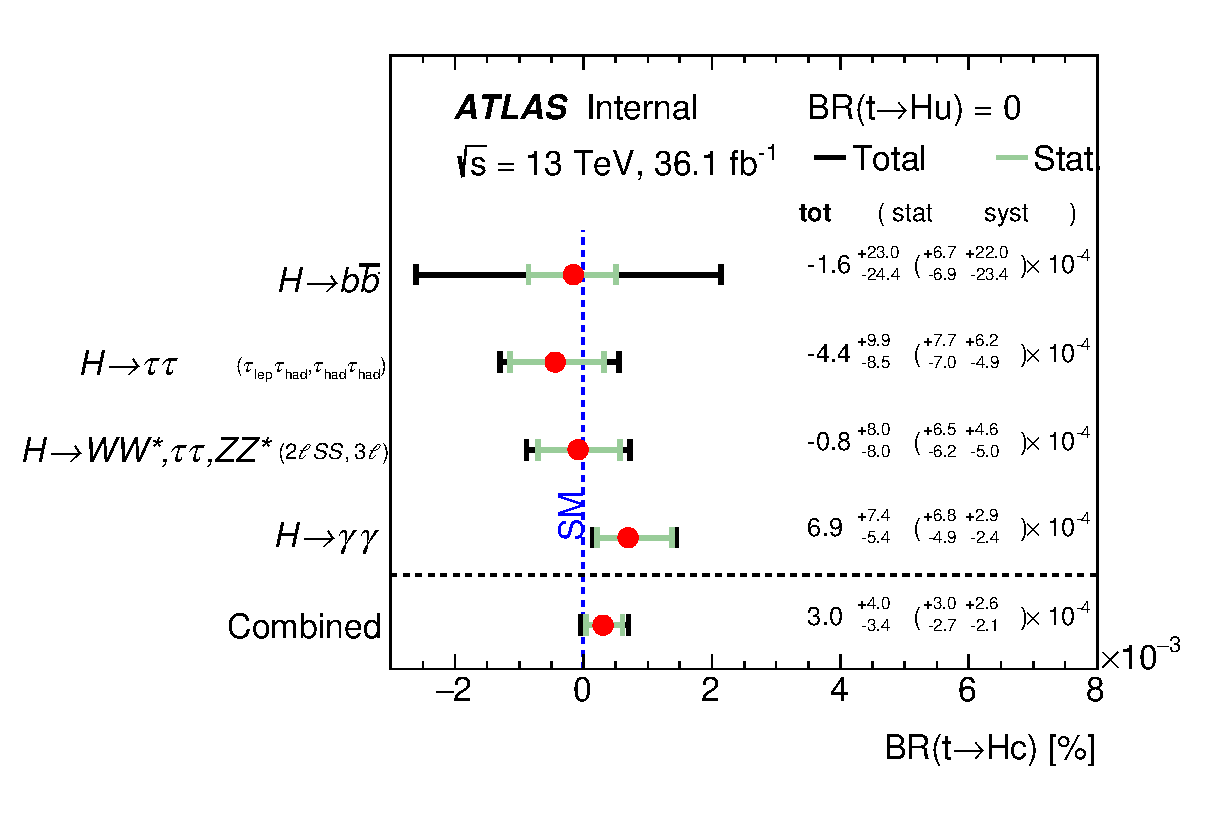
\includegraphics[width=0.6\textwidth]{figures/Combo/POI2.eps}
\caption{\small {Summary of the best-fit $\BR(t\to Hu)$ for the individual searches as well as their combination,
assuming that $\BR(t\to Hc)=0$. }}
\label{fig:summary_printnum_hu} 
\end{center}
\end{figure*}
%%%%%%%%%%%%%%

%%%%%%%%%%%%%%%
\begin{table}[t!]
\begin{center}
\begin{tabular}{lcc}
\toprule\toprule
 & \multicolumn{1}{c}{95\% CL upper limits} & \multicolumn{1}{c}{95\% CL upper limits}  \\
 & \multicolumn{1}{c}{on $\BR(t \to Hc)$} & \multicolumn{1}{c}{on $\BR(t \to Hu)$} \\
 &  Observed (Expected) & Observed (Expected)  \\
\midrule\midrule
$H \to b\bar{b}$ & $4.2 \times 10^{-3}$ ($4.0 \times 10^{-3}$) & $5.2 \times 10^{-3}$ ($4.9 \times 10^{-3}$) \\
$H \to \tau^+\tau^-$ ($\lephad$, $\hadhad$) & $1.9 \times 10^{-3}$ ($2.1 \times 10^{-3}$) & $1.7 \times 10^{-3}$ ($2.0 \times 10^{-3}$) \\ 
$H \to WW^*, \tau^+\tau^-, ZZ^*$ ($2\ell$SS, $3\ell$)~\cite{Aaboud:2018pob}  & $1.6 \times 10^{-3}$ ($1.5 \times 10^{-3}$) & $1.9 \times 10^{-3}$ ($1.5 \times 10^{-3}$) \\ 
$H \to \gamma\gamma$~\cite{Aaboud:2017mfd} & $2.2 \times 10^{-3}$ ($1.6 \times 10^{-3}$) & $2.4 \times 10^{-3}$ ($1.7 \times 10^{-3}$) \\
\midrule
Combination  & $1.1 \times 10^{-3}$ ($8.3 \times 10^{-4}$) & $1.2 \times 10^{-3}$ ($8.3 \times 10^{-4}$) \\
\bottomrule\bottomrule
\end{tabular}
\caption{\small{Summary of 95\% CL upper limits on $\BR(t \to Hq)$ from ATLAS searches based on 
36~$\ifb$ of data at $\sqrt{s}=13~\tev$. Signatures with two same-charge (three) light leptons and no $\tauhad$ candidates
are denoted as $2\ell$SS ($3\ell$). }}
\label{tab:limits_summary}
\end{center}
\end{table}
%%%%%%%%%%%%%%%

%%%%%%%%%%%%%%
\begin{figure*}[htbp]
\begin{center}
\subfloat[]{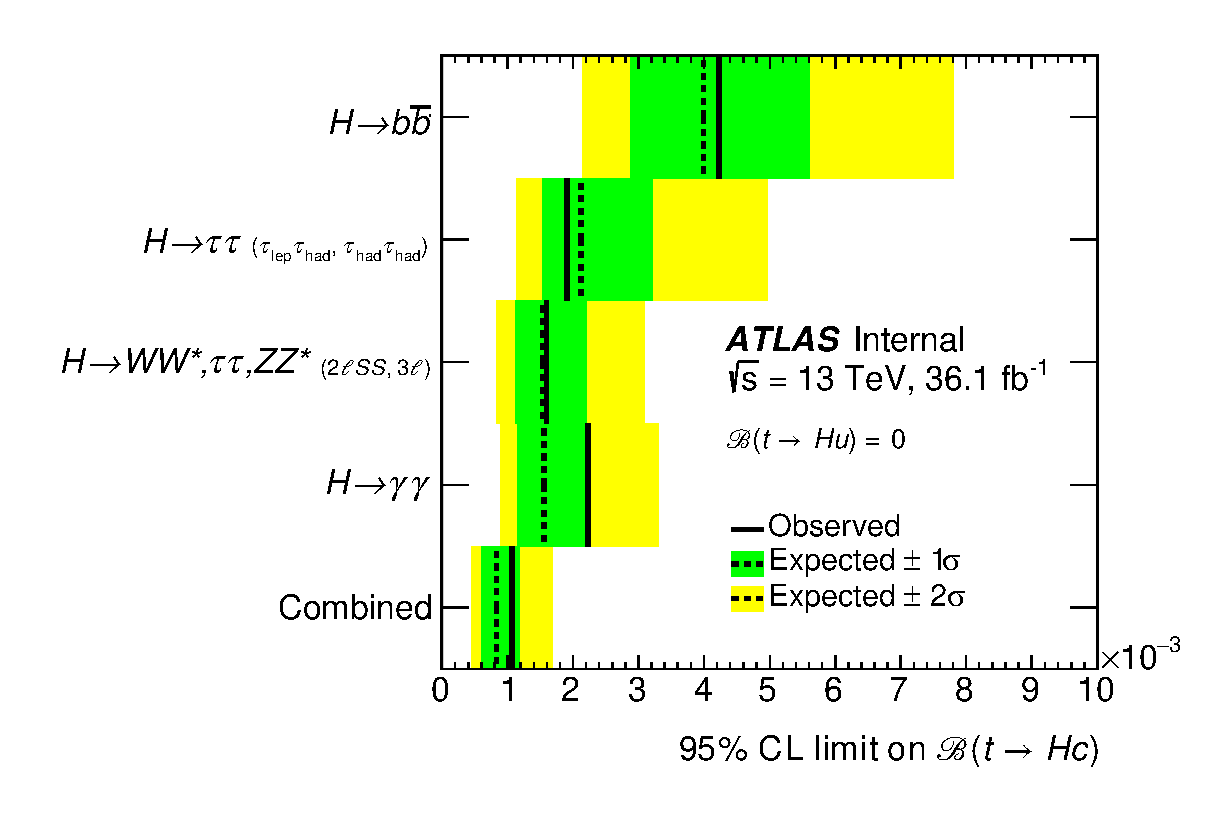
\includegraphics[width=0.49\textwidth]{figures/Combo/Limits.eps}}
\subfloat[]{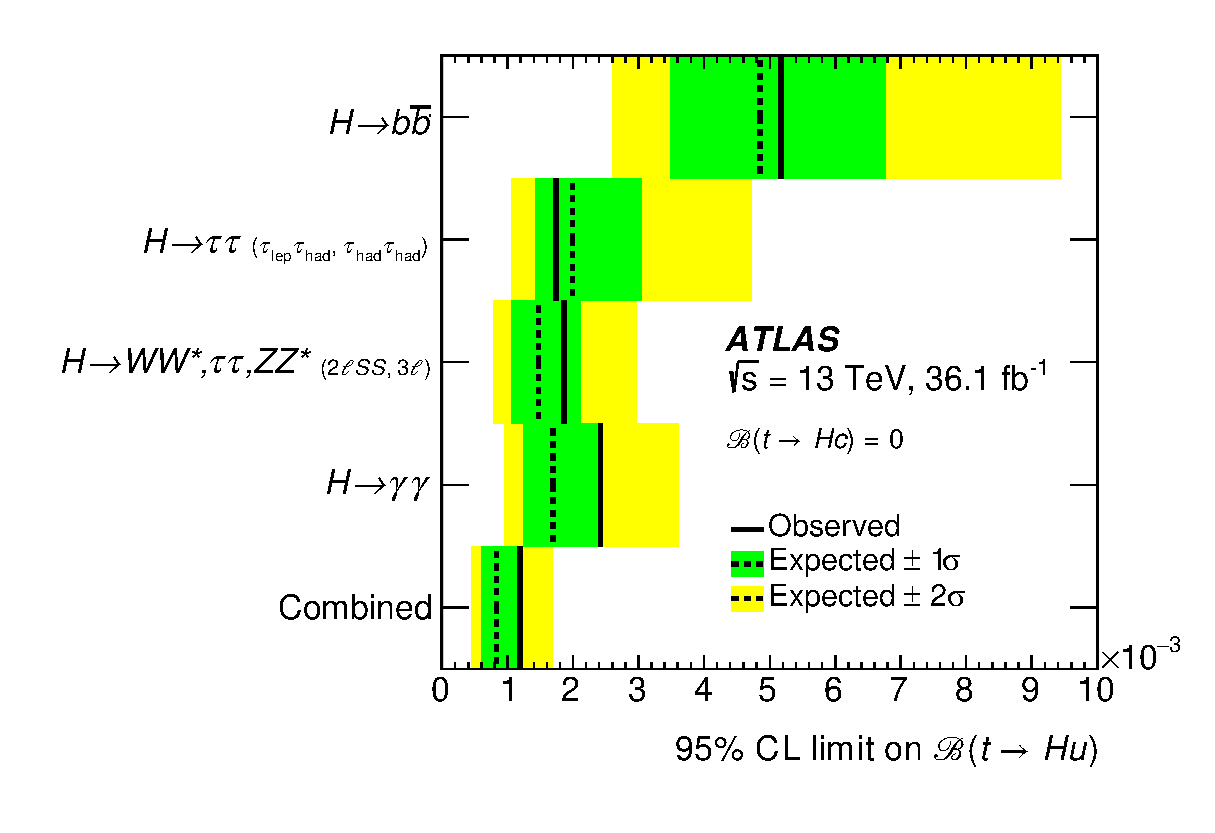
\includegraphics[width=0.49\textwidth]{figures/Combo/Limits2.eps}}
\caption{\small {95\% CL upper limits on (a) $\BR(t\to Hc)$ and (b) $\BR(t\to Hu)$ for the individual searches as well as their
combination, assuming that the other branching ratio is zero. The observed limits (solid lines) are compared to the 
expected (median) limits under the background-only
hypothesis (dotted lines). The surrounding shaded bands correspond to the 68\% and 95\% CL intervals around the expected limits, 
denoted by $\pm 1\sigma$ and $\pm 2\sigma$, respectively.
%Because the asymptotic approximation is used in the calculation of CL$_\mathrm{{s}}$, 
%the results of the $H \to\gamma\gamma$ search reported in this figure differ slightly from 
%those published in ref.~\cite{Aad:2014dya}, which remain the most accurate results.
}}
\label{fig:limits_combo_1D} 
\end{center}
\end{figure*}
%%%%%%%%%%%%%%

%%%%%%%%%%%%%%%
%\begin{figure*}[htbp]
%\begin{center}
%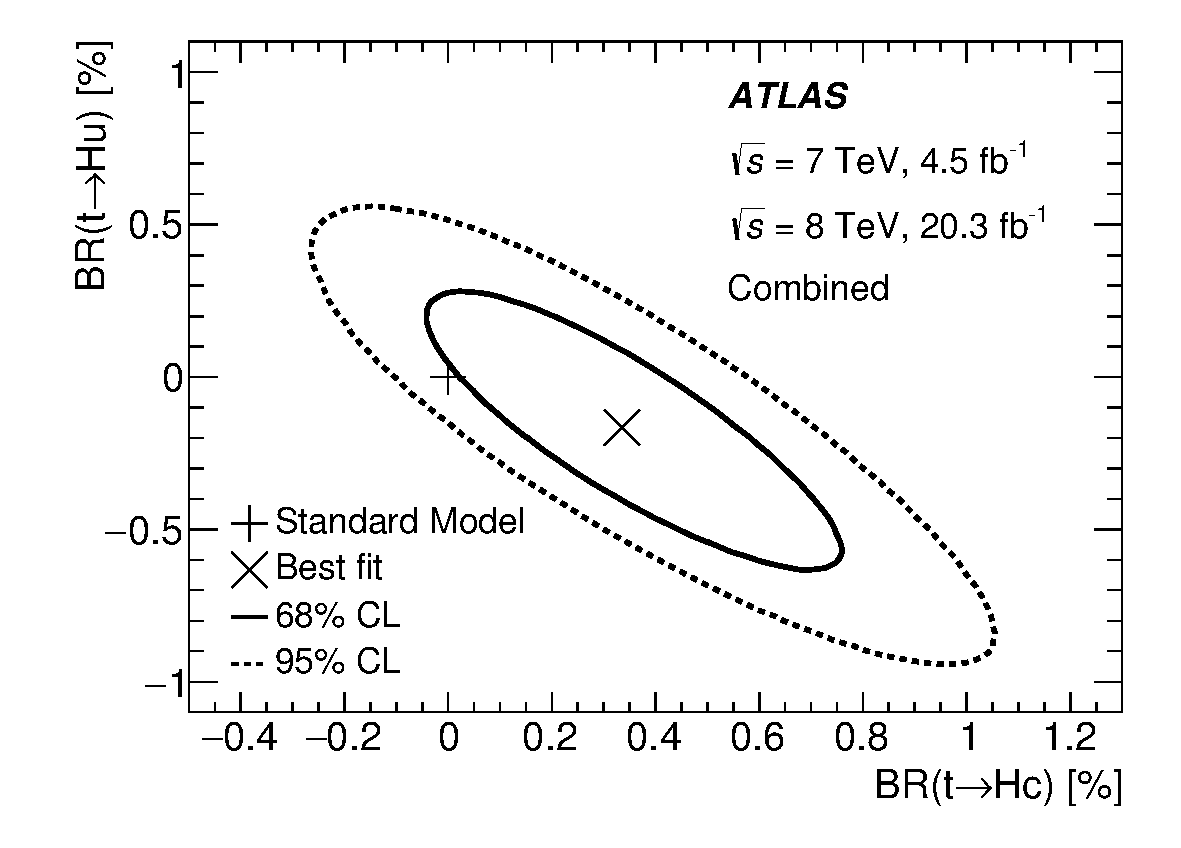
\includegraphics[width=0.49\textwidth]{figures/Combo/fig13.pdf}
%\caption{\small {
%Best-fit $\BR(t\to Hc)$ and $\BR(t\to Hu)$ and the corresponding 68\% CL (solid) and 95\% CL (dotted) regions for the combination of the searches.
%\textbf{TO UPDATE: placeholder figure from the Run 1 paper.}}}
%\label{fig:nllscan_combo_2D} 
%\end{center}
%\end{figure*}
%%%%%%%%%%%%%%%

%%%%%%%%%%%%%%
\begin{figure*}[htbp]
\begin{center}
\subfloat[]{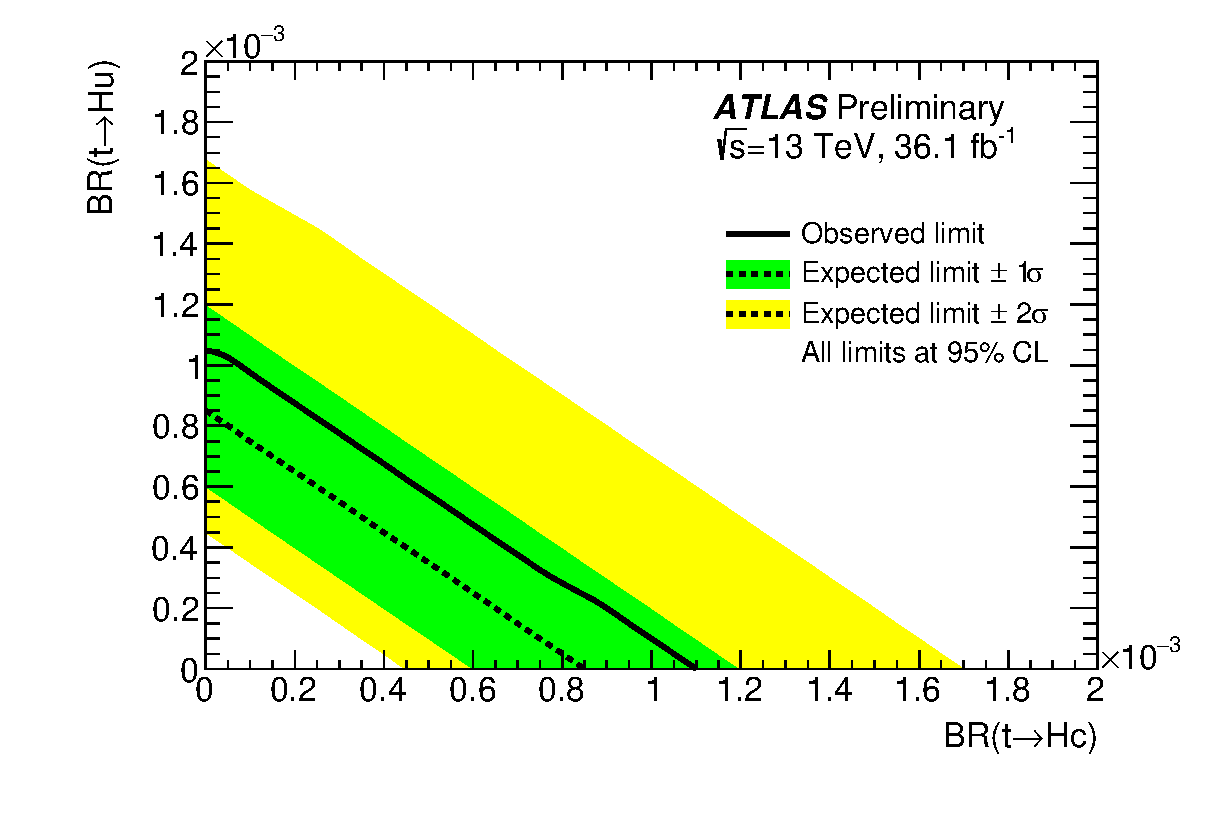
\includegraphics[width=0.49\textwidth]{figures/Combo/Limits2D.eps}}
\subfloat[]{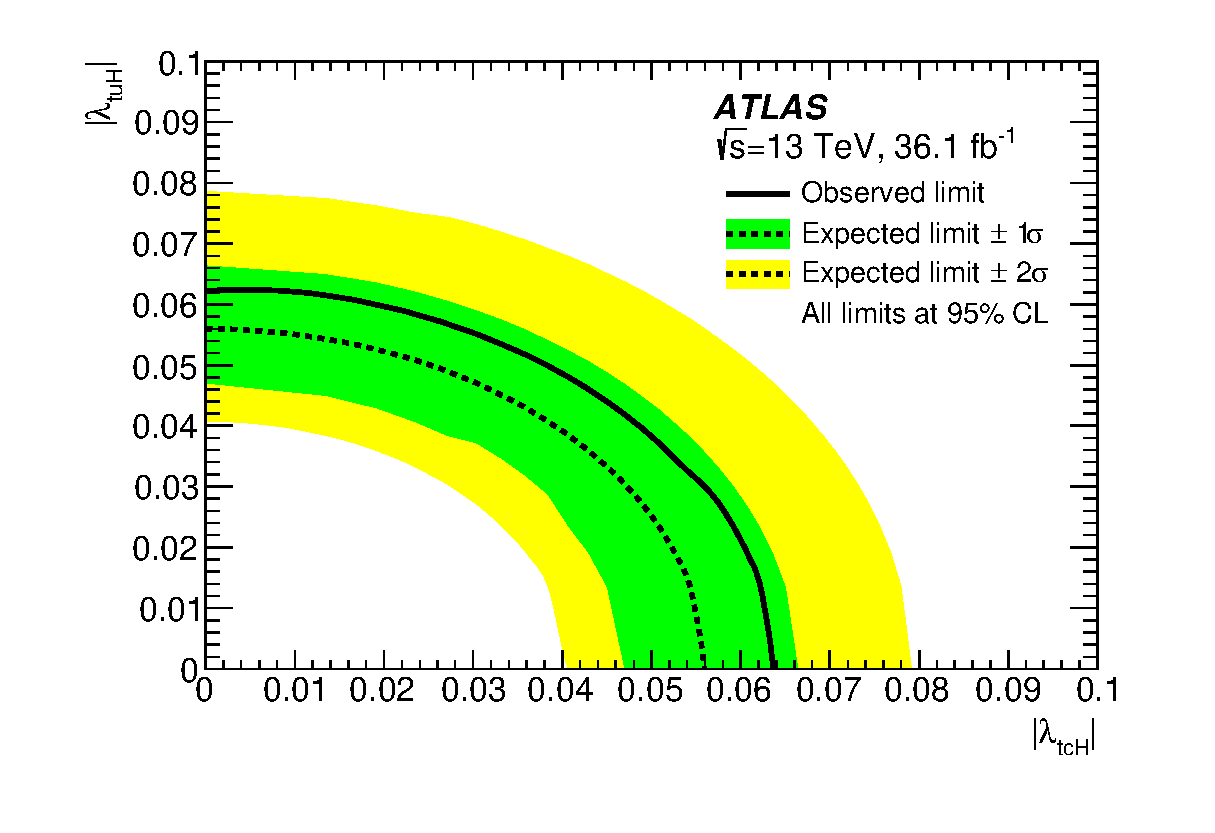
\includegraphics[width=0.49\textwidth]{figures/Combo/Coupling2D.eps}}
\caption{\small {95\% CL upper limits (a) on the plane of $\BR(t\to Hu)$ versus $\BR(t\to Hc)$ and (b) on the plane 
of $|\lamHu|$ versus $|\lamHc|$ for the combination of the searches. The observed limits (solid lines) are compared to the expected (median) limits under the background-only hypothesis (dotted lines). The surrounding shaded bands correspond to the 68\% and 95\% CL intervals around the expected limits, 
denoted by $\pm 1\sigma$ and $\pm 2\sigma$, respectively.}}
\label{fig:limits_combo_2D} 
\end{center}
\end{figure*}
%%%%%%%%%%%%%%

